% CS765A Advanced Programming in the UNIX Environment
% Author: Jan Schaumann <jschauma@netmeister.org>
% $Id: slides.tex,v 1.6 2005/08/30 21:43:10 jschauma Exp $
%\special{! TeXDict begin /landplus90{true}store end }

\documentclass[xga]{xdvislides}
\usepackage[landscape]{geometry}
\usepackage{graphics}
\usepackage{graphicx}
\usepackage{colordvi}
\usepackage{tabularx}

\begin{document}
\setfontphv

%%% Headers and footers
\lhead{\slidetitle}
\chead{CS631 - Advanced Programming in the UNIX Environment}
\rhead{Slide \thepage}
\lfoot{\Gray{Lecture 13: Review}}
\cfoot{\relax}
\rfoot{\Gray{\today}}

\vspace*{\fill}
\begin{center}
	\Hugesize
		CS631 - Advanced Programming in the UNIX Environment\\ [1em]
	\hspace*{5mm}\blueline\\ [1em]
	\Normalsize
		Department of Computer Science\\
		Stevens Institute of Technology\\
		Jan Schaumann\\
		\verb+jschauma@stevens.edu+\\
		\verb+http://www.cs.stevens.edu/~jschauma/631/+
\end{center}
\vspace*{\fill}

\subsection{In a nutshell: the "what"}
\begin{verbatim}
$ ls /bin
[          csh        ed         ls         pwd        sleep
cat        date       expr       mkdir      rcmd       stty
chio       dd         hostname   mt         rcp        sync
chmod      df         kill       mv         rm         systrace
cp         domainname ksh        pax        rmdir      tar
cpio       echo       ln         ps         sh         test
$
\end{verbatim}

\subsection{In a nutshell: the "what"}
\begin{verbatim}
$ grep "(int" /usr/include/sys/socket.h
int	accept(int, struct sockaddr * __restrict, socklen_t * __restrict);
int	bind(int, const struct sockaddr *, socklen_t);
int	connect(int, const struct sockaddr *, socklen_t);
int	getsockopt(int, int, int, void * __restrict, socklen_t * __restrict);
int	listen(int, int);
ssize_t	recv(int, void *, size_t, int);
ssize_t	recvfrom(int, void * __restrict, size_t, int,
ssize_t	recvmsg(int, struct msghdr *, int);
ssize_t	send(int, const void *, size_t, int);
ssize_t	sendto(int, const void *,
ssize_t	sendmsg(int, const struct msghdr *, int);
int	setsockopt(int, int, int, const void *, socklen_t);
int	socket(int, int, int);
int	socketpair(int, int, int, int *);
$
\end{verbatim}

\subsection{In a nutshell: the "what"}
\begin{itemize}
	\item gain an understanding of the UNIX operating systems
	\item gain (systems) programming experience
	\item understand fundamental OS concepts (with focus on UNIX family):
		\begin{itemize}
			\item multi-user concepts
			\item basic and advanced I/O
			\item process relationships
			\item interprocess communication
			\item basic network programming using a client/server model
		\end{itemize}
\end{itemize}

\subsection{In a nutshell: the "how"}
\small
\begin{verbatim}

    static char dot[] = ".", *dotav[] = { dot, NULL };
    struct winsize win;
    int ch, fts_options;
    int kflag = 0;
    const char *p;

    setprogname(argv[0]);
    setlocale(LC_ALL, "");

    /* Terminal defaults to -Cq, non-terminal defaults to -1. */
    if (isatty(STDOUT_FILENO)) {
        if (ioctl(STDOUT_FILENO, TIOCGWINSZ, &win) == 0 &&
            win.ws_col > 0)
            termwidth = win.ws_col;
        f_column = f_nonprint = 1;
    } else
        f_singlecol = 1;

    /* Root is -A automatically. */
    if (!getuid())
        f_listdot = 1;

    fts_options = FTS_PHYSICAL;
    while ((ch = getopt(argc, argv, "1ABCFLRSTWabcdfghiklmnopqrstuwx")) != -1) {
        switch (ch) {
        /*
         * The -1, -C, -l, -m and -x options all override each other so
         * shell aliasing works correctly.
         */
        case '1':
            f_singlecol = 1;
\end{verbatim}
\Normalsize

\subsection{Programming}
\begin{center}
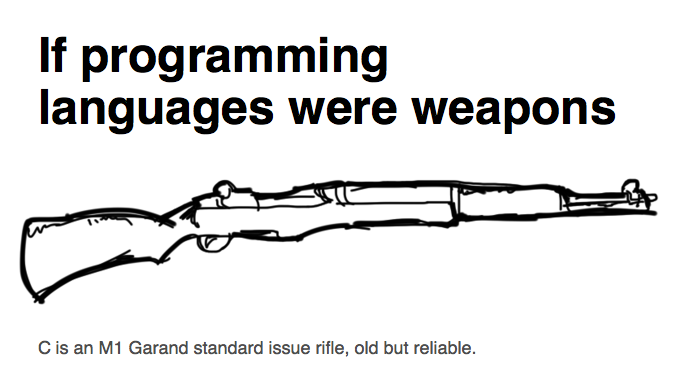
\includegraphics[scale=0.7,angle=-90]{pics/if-programming-languages-were-weapons.eps} \\
\vspace{.5in}
\verb+http://is.gd/6aidgb+ \\
\verb+https://i.imgur.com/ZyeCO.jpg+
\end{center}


\subsection{UNIX Basics: Architecture}
\begin{center}
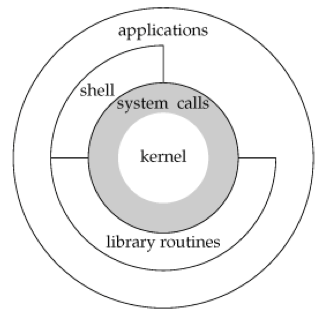
\includegraphics[angle=-90]{pics/unix_architecture.eps}
\end{center}

\subsection{UNIX Basics: Pipelines}
Say "Thank you, Douglas McIlroy!"
\begin{center}
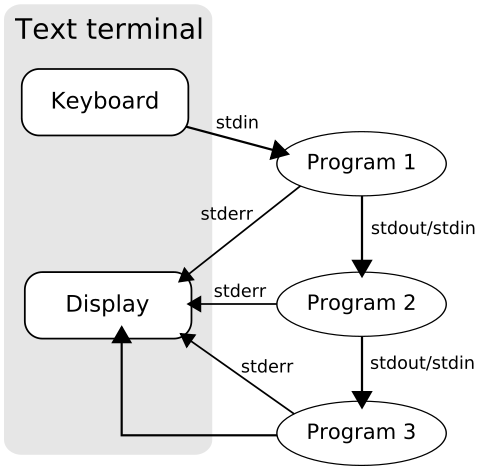
\includegraphics[scale=0.65,angle=-90]{pics/pipeline.eps} \\
\verb+http://is.gd/vGHO9J+ \\
\end{center}

\subsection{Program Design}
\vspace*{\fill}
\Huge
\begin{center}
"Consistency underlies all principles of quality." Frederick P. Brooks, Jr
\end{center}
\Normalsize
\vspace*{\fill}


\subsection{Program Design}
\verb+https://secure.wikimedia.org/wikipedia/en/wiki/Unix_philosophy+ \\

UNIX programs...
\begin{itemize}
	\item ...are simple
	\item ...have a manual page
	\item ...follow the element of least surprise
	\item ...accept input from {\tt stdin}
	\item ...generate output to {\tt stdout}
	\item ...generate meaningful error messages to {\tt stderr}
	\item ...have meaningful exit codes
\end{itemize}


\subsection{Files and Directories}
\begin{itemize}
	\item The UNIX {\bf filesystem} is a tree structure, with all partitions
		mounted under the root (/). File names may consist of any
		character except / and NUL as pathnames are a sequence of
		zero or more filenames separated by /'s.
	\item Directories are special "files" that contain mappings
		between {\em inodes} and {\em filenames}, called directory
		entries.
	\item All processes have a current working directory from which
		all relative paths are specified. (Absolute paths begin
		with a slash, relative paths do not.)
\end{itemize}

\subsection{User Identification}
\begin{itemize}
	\item {\em User ID}s and {\em group ID}s are numeric values used to
		identify users on the system and grant permissions appropriate to them.
	\item {\em Group ID}s come in two types; {\em primary} and {\em secondary}.
\end{itemize}

\subsection{Unix Time Values}
{\em Calendar time}: measured in seconds since the UNIX epoch (Jan
1, 00:00:00, 1970, GMT). Stored in a variable of type {\tt time\_t}.
\\

\begin{center}

\includegraphics[scale=0.8,angle=-90]{pics/epoch-fail.eps} \\
\verb+https://www.xkcd.com/376/+ \\
\vspace{.25in}
\verb+https://secure.wikimedia.org/wikipedia/en/wiki/Year_2038_problem+
\end{center}


\subsection{Unix Time Values}
{\em Process time}: central processor resources used by a process.
Measured in {\em clock ticks} ({\tt clock\_t}).  Three values:
\begin{itemize}
	\item clock time
	\item user CPU time
	\item system CPU time
\end{itemize}

\vspace*{\fill}
\begin{verbatim}
$ time grep -r _POSIX_SOURCE /usr/include >/dev/null
\end{verbatim}
\vspace*{\fill}

\subsection{Standard I/O}
\begin{itemize}
	\item	Standard I/O:
		\begin{itemize}
			\item {\bf file descriptors}: Small, non-negative
				integers which identify a file to the kernel.
				The shell can redirect any file descriptor.
			\item kernel provides {\bf unbuffered} I/O through e.g.
				{\tt open read write lseek close}
			\item kernel provides {\bf buffered} I/O through e.g.
				{\tt getc putc fopen fread fwrite}
		\end{itemize}
\end{itemize}

\subsection{Processes}
Programs executing in memory are called {\em processes}.
\begin{itemize}
	\item Programs are brought into memory via one of the
		six {\tt exec(3)} functions.  Each process is identified
		by a guaranteed unique non-negative integer called the
		{\em processes ID}. New processes can {\bf only} be
		created via the {\tt fork(2)} system call.
	\item {\bf process control} is performed mainly by the
		{\tt fork(2)}, {\tt exec(3)} and {\tt waitpid(2)} functions.
\end{itemize}

\subsection{Processes}
\begin{center}
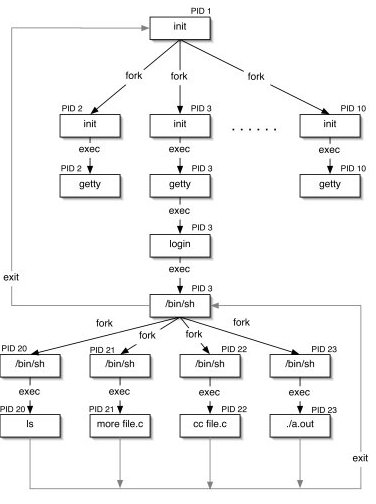
\includegraphics[scale=0.75]{pics/process-tree.eps} \\
\end{center}

\subsection{Processes}
\vspace*{\fill}
\Huge
\begin{center}
	{\tt \$ pstree -hapun | more}
\end{center}
\Normalsize
\vspace*{\fill}

\subsection{Important ANSI C Features, Error Handling}
\begin{itemize}
	\item	Important ANSI C Features:
		\begin{itemize}
			\item function prototypes
			\item generic pointers ({\tt void *})
			\item abstract data types (e.g. {\tt pid\_t}, {\tt size\_t})
		\end{itemize}
	\item	Error Handling:
		\begin{itemize}
			\item meaningful return values
			\item {\tt errno} variable
			\item look up constant error values via two functions:
				\small
				\setlength{\unitlength}{1mm}
				\begin{center}
					\begin{picture}(200,20)
						\thinlines
						\put(-10,0){\framebox(180,15){}}
						\put(0,10){{\tt \#include <string.h>}}
						\put(0,5){{\tt char *strerror(int {\em errnum})}}
						\put(100,2){Returns: pointer to message string}
					\end{picture}
					\begin{picture}(200,20)
						\thinlines
						\put(-10,0){\framebox(180,15){}}
						\put(0,10){{\tt \#include <stdio.h>}}
						\put(0,5){{\tt void perror(const char {\em *msg})}}
					\end{picture}
				\end{center}
		\end{itemize}
\end{itemize}

\newpage

\vspace*{\fill}
\begin{center}
  \Hugesize
    Lecture 02
	\hspace*{5mm}\blueline\\ [1em]
	File I/O, File Sharing
  \Normalsize
\end{center}
\vspace*{\fill}

\subsection{File Descriptors}
\begin{itemize}
	\item A {\em file descriptor} (or {\em file handle}) is a small,
		non-negative integer which identifies a file to the kernel.
	\item Traditionally, {\tt stdin}, {\tt stdout} and {\tt stderr}
		are 0, 1 and 2 respectively.
	\item Relying on ``magic numbers'' is Bad\texttrademark.  Use {\tt
		STDIN\_FILENO}, {\tt STDOUT\_FILENO} and {\tt STDERR\_FILENO}.
\end{itemize}
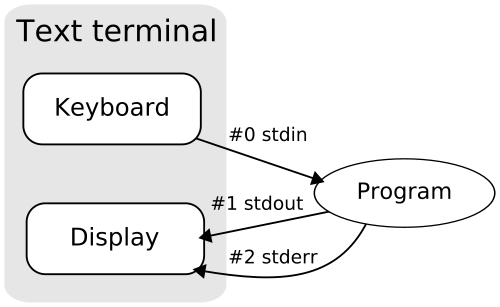
\includegraphics[scale=0.5,angle=-90]{pics/stdstreams.eps}
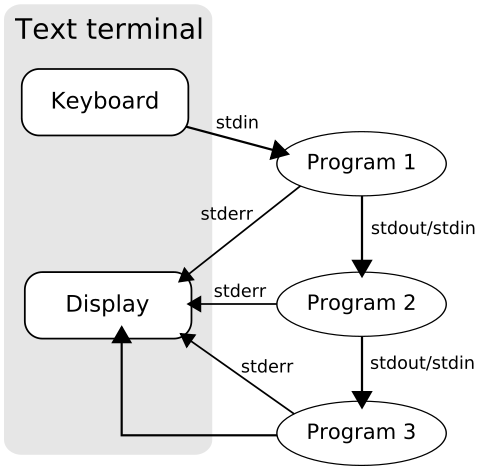
\includegraphics[scale=0.4,angle=-90]{pics/pipeline.eps}

\subsection{Standard I/O}
Basic File I/O: almost all UNIX file I/O can be
performed using these five functions:
\begin{itemize}
	\item {\tt open(2)}
	\item {\tt close(2)}
	\item {\tt lseek(2)}
	\item {\tt read(2)}
	\item {\tt write(2)}
\end{itemize}
\vspace{.25in}
Processes may want to share recources.  This requires us to look at:
\begin{itemize}
	\item atomicity of these operations
	\item file sharing
	\item manipulation of file descriptors
\end{itemize}

\subsection{{\tt open(2)}}
\small
\setlength{\unitlength}{1mm}
\begin{center}
	\begin{picture}(200,25)
		\thinlines
		\put(0,0){\framebox(180,25){}}
		\put(10,20){{\tt \#include <fcntl.h>}}
		\put(10,12){{\tt int open(const char *{\em pathname}, int {\em oflag}, ... /* mode\_t {\em mode} */ );}}
		\put(115,3){Returns:  file descriptor if OK, -1 on error}
	\end{picture}
\end{center}
\vspace{.25in}
\Normalsize
{\em oflag} must be one (and only one) of:
\small
\begin{itemize}
	\item {\tt O\_RDONLY} -- Open for reading only
	\item {\tt O\_WRONLY} -- Open for writing only
	\item {\tt O\_RDWR} -- Open for reading and writing
\end{itemize}
\vspace{.25in}
\Normalsize
and may be OR'd with any of these:
\small
\begin{itemize}
	\item {\tt O\_APPEND} -- Append to end of file for each write
	\item {\tt O\_CREAT} -- Create the file if it doesn't exist. Requires
		{\em mode} argument
	\item {\tt O\_EXCL} -- Generate error if {\tt O\_CREAT} and file
		already exists. (atomic)
	\item {\tt O\_TRUNC} -- If file exists and successfully open in
		{\tt O\_WRONLY} or {\tt O\_RDWR}, make length = 0
	\item {\tt O\_NOCTTY} -- If pathname refers to a terminal device, do
		not allocate the device as a controlling terminal
	\item {\tt O\_NONBLOCK} -- If pathname refers to a FIFO, block special,
		or char special, set nonblocking mode (open and I/O)
	\item {\tt O\_SYNC} --  Each write waits for physical I/O to complete
\end{itemize}

\subsection{{\tt open(2)} variants}
\small
\setlength{\unitlength}{1mm}
\begin{center}
	\begin{picture}(200,28)
		\thinlines
		\put(0,0){\framebox(180,28){}}
		\put(10,23){{\tt \#include <fcntl.h>}}
		\put(10,15){{\tt int open(const char *{\em pathname}, int {\em oflag}, ... /* mode\_t {\em mode} */ );}}
		\put(10,10){{\tt int openat(int {\em dirfd}, const char *{\em pathname}, int {\em oflag}, ... /* mode\_t {\em mode} */ );}}
		\put(115,3){Returns:  file descriptor if OK, -1 on error}
	\end{picture}
\end{center}
\vspace{.25in}
\Normalsize
On some platforms {\em oflag} may also be one of:
\small
\begin{itemize}
	\item {\tt O\_EXEC} -- Open for execute only
	\item {\tt O\_SEARCH} -- Open for search only (applies to directories)
\end{itemize}
\vspace{.25in}
\Normalsize
and may be OR'd with any of these:
\small
\begin{itemize}
	\item {\tt O\_DIRECTORY} -- If path resolves to a non-directory file, fail and set errno to {\tt ENOTDIR}.
	\item {\tt O\_DSYNC} -- Wait for physical I/O for data, except
file attributes
	\item {\tt O\_RSYNC} -- Block read operations on any pending writes.
	\item {\tt O\_PATH} -- Obtain a file descriptor purely for
fd-level operations. (Linux $>$2.6.36 only)
\end{itemize}
\Normalsize
\vspace{.25in}
{\tt openat(2)} is used to handle relative pathnames from different
working directories in an atomic fashion.


\subsection{{\tt close(2)}}
\small
\setlength{\unitlength}{1mm}
\begin{center}
	\begin{picture}(200,25)
		\thinlines
		\put(0,0){\framebox(180,25){}}
		\put(10,20){{\tt \#include <unistd.h>}}
		\put(10,10){{\tt int close(int {\em fd});}}
		\put(115,3){Returns:  0 if OK, -1 on error}
	\end{picture}
\end{center}
\Normalsize
\vspace{.25in}
\begin{itemize}
	\item closing a filedescriptor releases any record locks on
		that file (more on that in future lectures)
	\item file descriptors not explicitly closed are closed by the kernel
		when the process terminates.
\end{itemize}

\subsection{{\tt read(2)}}
\small
\setlength{\unitlength}{1mm}
\begin{center}
	\begin{picture}(200,25)
		\thinlines
		\put(0,0){\framebox(180,25){}}
		\put(10,20){{\tt \#include <unistd.h>}}
		\put(10,12){{\tt ssize\_t read(int {\em filedes}, void *{\em buff}, size\_t {\em nbytes} );}}
		\put(85,3){Returns:  number of bytes read, 0 if end of file, -1 on error}
	\end{picture}
\end{center}
\Normalsize
There can be several cases where {\tt read} returns less than the number of
bytes requested:
\begin{itemize}
	\item EOF reached before requested number of bytes have been read
	\item Reading from a terminal device, one "line" read at a time
	\item Reading from a network, buffering can cause delays in arrival of data
	\item Record-oriented devices (magtape) may return data one record at
		a time
	\item Interruption by a signal
\end{itemize}
\vspace{.25in}
{\tt read} begins reading at the current offset, and increments the offset
by the number of bytes actually read.
% Note that {\tt ssize\_t} is a signed
% type, while {\tt size\_t} is unsigned.

\subsection{{\tt write(2)}}
\small
\setlength{\unitlength}{1mm}
\begin{center}
	\begin{picture}(200,25)
		\thinlines
		\put(0,0){\framebox(180,25){}}
		\put(10,20){{\tt \#include <unistd.h>}}
		\put(10,12){{\tt ssize\_t write(int {\em filedes}, void *{\em buff}, size\_t {\em nbytes} );}}
		\put(85,3){Returns:  number of bytes written if OK, -1 on error}
	\end{picture}
\end{center}
\Normalsize
\vspace{.25in}
\begin{itemize}
	\item {\tt write} returns {\tt nbytes} or an error has occurred (disk
		full, file size limit exceeded, ...)
	\item for regular files, {\tt write} begins writing at the
		current offset (unless {\tt O\_APPEND} has been specified, in which
		case the offset is first set to the end of the file)
	\item after the write, the offset is
		adjusted by the number of bytes actually written
\end{itemize}

\subsection{{\tt lseek(2)}}
\small
\setlength{\unitlength}{1mm}
\begin{center}
	\begin{picture}(200,30)
		\thinlines
		\put(0,0){\framebox(180,30){}}
		\put(10,25){{\tt \#include <sys/types.h>}}
		\put(10,20){{\tt \#include <fcntl.h>}}
		\put(10,12){{\tt off\_t lseek(int {\em filedes}, off\_t {\em offset}, int {\em whence} );}}
		\put(115,3){Returns:  new file offset if OK, -1 on error}
	\end{picture}
\end{center}
\Normalsize
\vspace{.25in}
The value of whence determines how offset is used:
\small
\begin{itemize}
	\item {\tt SEEK\_SET} bytes from the beginning of the file
	\item {\tt SEEK\_CUR} bytes from the current file position
	\item {\tt SEEK\_END} bytes from the end of the file
\end{itemize}
\Normalsize
\vspace{.25in}
``Weird'' things you can do using {\tt lseek(2)}:
\begin{itemize}
	\item seek to a negative offset
	\item seek 0 bytes from the current position
	\item seek past the end of the file
\end{itemize}

\subsection{File Sharing}
Since UNIX is a multi-user/multi-tasking system, it is conceivable (and useful)
if more than one process can act on a single file simultaneously. In
order to understand how this is accomplished, we need to examine some kernel
data structures which relate to files.  (See: Stevens, pp 70 ff)

\begin{itemize}
	\item each process table entry has a table of file descriptors, which
		contain
		\begin{itemize}
			\item the file descriptor flags (ie {\tt FD\_CLOEXEC}, see \verb+fcntl(2)+)
			\item a pointer to a file table entry
		\end{itemize}
	\item the kernel maintains a file table;  each entry contains
		\begin{itemize}
			\item file status flags (\verb+O_APPEND+, \verb+O_SYNC+, \verb+O_RDONLY+, etc.)
			\item current offset
			\item pointer to a vnode table entry
		\end{itemize}
	\item a vnode structure contains
		\begin{itemize}
			\item vnode information
			\item inode information (such as current file size)
		\end{itemize}
\end{itemize}

\subsection{File Sharing}
\begin{center}
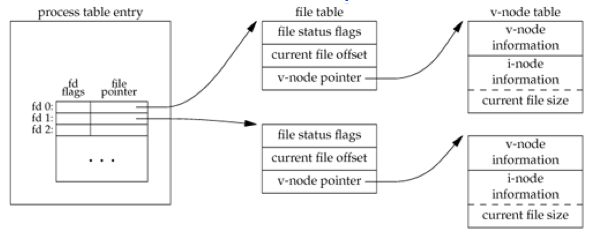
\includegraphics[scale=0.8,angle=-90]{pics/open-files.eps} \\
\end{center}

\subsection{File Sharing}
Knowing this, here's what happens with each of the calls we discussed earlier:

\begin{itemize}
	\item after each {\tt write} completes, the current file offset in the
		file table entry is incremented.  (If current\_file\_offset $>$
		current\_file\_size, change current file size in i-node table entry.)
	\item If file was opened {\tt O\_APPEND} set corresponding flag in file status
		flags in file table. For each {\tt write}, current file offset is first set to
		current file size from the i-node entry.
	\item {\tt lseek} simply adjusts current file offset in file table entry
	\item to {\tt lseek} to the end of a file, just copy current file size into
		current file offset.
\end{itemize}

\subsection{{\tt dup(2)} and {\tt dup2(2)}}
\small
\setlength{\unitlength}{1mm}
\begin{center}
	\begin{picture}(150,30)
		\thinlines
		\put(0,0){\framebox(130,30){}}
		\put(10,25){{\tt \#include <unistd.h>}}
		\put(10,17){{\tt int dup(int {\em oldd});}}
		\put(10,12){{\tt int dup2(int {\em oldd}, int {\em newd});}}
		\put(55,3){Both return new file descriptor if OK, -1 on error}
	\end{picture}
\end{center}
\Normalsize

An existing file descriptor can be duplicated with {\tt dup(2)} or duplicated to
a particular file descriptor value with {\tt dup2(2)}. As with {\tt open(2)}, {\tt
dup(2)} returns the lowest numbered unused file descriptor.
\\

Note the difference in scope of the file {\em descriptor} flags and the
file {\em status} flags compared to distinct processes.
\begin{center}
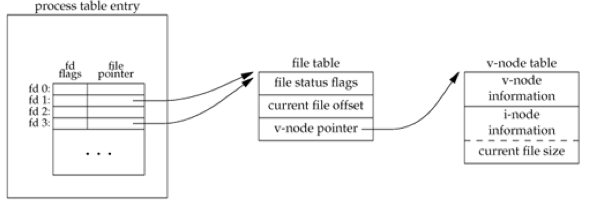
\includegraphics[scale=0.7,angle=-90]{pics/dup.eps} \\
\end{center}

\newpage

\vspace*{\fill}
\begin{center}
  \Hugesize
    Lecture 03
	\hspace*{5mm}\blueline\\ [1em]
	Files and Directories
  \Normalsize
\end{center}
\vspace*{\fill}

\subsection{{\tt stat(2)} family of functions}
\small
\setlength{\unitlength}{1mm}
\begin{center}
	\begin{picture}(150,40)
		\thinlines
		\put(0,0){\framebox(130,40){}}
		\put(10,35){{\tt \#include <sys/types.h>}}
		\put(10,30){{\tt \#include <sys/stat.h>}}
		\put(10,22){{\tt int stat(const char *{\em path}, struct stat *{\em sb});}}
		\put(10,18){{\tt int lstat(const char *{\em path}, struct stat *{\em sb});}}
		\put(10,14){{\tt int fstat(int {\em fd}, struct stat *{\em sb});}}
		\put(85,3){Returns: 0 if OK, -1 on error}
	\end{picture}
\end{center}
\Normalsize

All these functions return extended attributes about the referenced file (in
the case of {\em symbolic links}, {\tt lstat(2)} returns attributes of the
{\em link}, others return stats of the referenced file).
\vspace{.25in}
\small
\begin{verbatim}
struct stat {
    dev_t      st_dev;          /* device number (filesystem) */
    ino_t      st_ino;          /* i-node number (serial number) */
    mode_t     st_mode;         /* file type & mode (permissions) */
    dev_t      st_rdev;         /* device number for special files */
    nlink_t    st_nlink;        /* number of links */
    uid_t      st_uid;          /* user ID of owner */
    gid_t      st_gid;          /* group ID of owner */
    off_t      st_size;         /* size in bytes, for regular files */
    time_t     st_atime;        /* time of last access */
    time_t     st_mtime;        /* time of last modification */
    time_t     st_ctime;        /* time of last file status change */
    long       st_blocks;       /* number of 512-byte* blocks allocated */
    long       st_blksize;      /* best I/O block size */
};
\end{verbatim}
\Normalsize

\subsection{{\tt struct stat}: {\tt st\_mode}}

The {\tt st\_mode} field of the {\tt struct stat} encodes the type of file:

\begin{itemize}
	\item {\bf regular} -- most common, interpretation of data is up to
		application
	\item {\bf directory} -- contains names of other files and pointer to
		information on those files. Any process can read, only kernel
		can write.
	\item {\bf character special} -- used for certain types of devices
	\item {\bf block special} -- used for disk devices (typically). All
		devices are either {\em character} or {\em block special}.
	\item {\bf FIFO} -- used for interprocess communication
		(sometimes called {\em named pipe})
	\item {\bf socket} -- used for network communication and non-network
		communication (same host).
	\item {\bf symbolic link} -- Points to another file.
\end{itemize}
\vspace{.25in}
Find out more in {\tt <sys/stat.h>}.

\subsection{{\tt struct stat}: {\tt st\_mode}, {\tt st\_uid} and {\tt st\_gid}}
Every process has six or more IDs associated with it:
\\

\begin{tabular}{| l | l |}
	\hline
	real user ID & who we really are \\
	real group ID & \\
	\hline
	effective user ID & used for file access permission checks \\
	effective group ID & \\
	supplementary group IDs & \\
	\hline
	saved set-user-ID & saved by {\tt exec} functions \\
	saved set-group-ID & \\
	\hline
\end{tabular}
\vspace{.25in}

Whenever a file is {\em setuid}, set the {\em effective user ID} to {\tt
st\_uid}. Whenever a file is {\em setgid}, set the {\em effective group ID} to
{\tt st\_gid}.  {\tt st\_uid} and {\tt st\_gid} always specify the owner and
group owner of a file, regardless of whether it is setuid/setgid.

\subsection{{\tt struct stat}: {\tt st\_mode}}
{\tt st\_mode} also encodes the file access permissions ({\tt S\_IRUSR},
{\tt S\_IWUSR}, {\tt S\_IXUSR}, {\tt S\_IRGRP}, {\tt S\_IWGRP}, {\tt S\_IXGRP},
{\tt S\_IROTH}, {\tt S\_IWOTH}, {\tt S\_IXOTH}).  Uses of the permissions are
summarized as follows:

\begin{itemize}
	\item To open a file, need execute permission on each directory component of the path
	\item To open a file with {\tt O\_RDONLY} or {\tt O\_RDWR}, need read permission
	\item To open a file with {\tt O\_WRONLY} or {\tt O\_RDWR}, need write permission
	\item To use {\tt O\_TRUNC}, must have write permission
	\item To create a new file, must have write+execute permission for the directory
	\item To delete a file, need write+execute on directory, file doesn't matter
	\item To execute a file (via {\tt exec} family), need execute permission
\end{itemize}

\subsection{{\tt struct stat}: {\tt st\_mode}}
Which permission set to use is determined (in order listed):
\begin{enumerate}
	\item If effective-uid == 0, grant access
	\item If effective-uid == {\tt st\_uid}
		\begin{enumerate}
			\item if appropriate user permission bit is set, grant access
			\item else, deny access
		\end{enumerate}
	\item If effective-gid == {\tt st\_gid}
		\begin{enumerate}
			\item if appropriate group permission bit is set, grant access
			\item else, deny access
		\end{enumerate}
	\item If appropriate other permission bit is set, grant access, else deny access
\end{enumerate}

\subsection{{\tt struct stat}: {\tt st\_mode}}
Ownership of {\bf new} files and directories:
\begin{itemize}
	\item {\tt st\_uid} = effective-uid
	\item {\tt st\_gid} = ...either:
		\begin{itemize}
			\item effective-gid of process
			\item gid of directory in which it is being created
		\end{itemize}
\end{itemize}

\subsection{{\tt umask(2)}}
\small
\setlength{\unitlength}{1mm}
\begin{center}
	\begin{picture}(150,25)
		\thinlines
		\put(0,0){\framebox(130,25){}}
		\put(10,20){{\tt \#include <sys/stat.h>}}
		\put(10,12){{\tt mode\_t umask(mode\_t {\em numask});}}
		\put(62,3){Returns: previous file mode creation mask}
	\end{picture}
\end{center}
\Normalsize

{\tt umask(2)} sets the file creation mode mask. Any bits that are {\em on} in
the file creation mask are turned {\em off} in the file's mode.
\\

Important because a user can set a default umask. If a program needs to be
able to insure certain permissions on a file, it may need to turn off (or
modify) the umask, which affects only the current process.

\subsection{{\tt chmod(2)}, {\tt lchmod(2)} and {\tt fchmod(2)}}
\small
\setlength{\unitlength}{1mm}
\begin{center}
	\begin{picture}(150,35)
		\thinlines
		\put(0,0){\framebox(130,35){}}
		\put(10,30){{\tt \#include <sys/stat.h>}}
		\put(10,22){{\tt int chmod(const char *{\em path}, mode\_t {\em mode});}}
		\put(10,17){{\tt int lchmod(const char *{\em path}, mode\_t {\em mode});}}
		\put(10,12){{\tt int fchmod(int {\em fd}, mode\_t {\em mode});}}
		\put(85,3){Returns: 0 if OK, -1 on error}
	\end{picture}
\end{center}
\Normalsize

Changes the permission bits on the file. Must be either superuser or {\em
effective uid} == {\tt st\_uid}. {\em mode} can be any of the bits from our
discussion of {\tt st\_mode} as well as:
\begin{itemize}
	\item {\tt S\_ISUID} -- setuid
	\item {\tt S\_ISGID} -- setgid
	\item {\tt S\_ISVTX} -- sticky bit (aka ``saved text'')
	\item {\tt S\_IRWXU} -- user read, write and execute
	\item {\tt S\_IRWXG} -- group read, write and execute
	\item {\tt S\_IRWXO} -- other read, write and execute
\end{itemize}

\subsection{{\tt chown(2)}, {\tt lchown(2)} and {\tt fchown(2)}}
\small
\setlength{\unitlength}{1mm}
\begin{center}
	\begin{picture}(150,35)
		\thinlines
		\put(0,0){\framebox(130,35){}}
		\put(10,30){{\tt \#include <unistd.h>}}
		\put(10,22){{\tt int chown(const char *{\em path}, uid\_t {\em owner}, gid\_t {\em group});}}
		\put(10,17){{\tt int lchown(const char *{\em path}, uid\_t {\em owner}, gid\_t {\em group});}}
		\put(10,12){{\tt int fchown(int {\em fd}, uid\_t {\em owner}, gid\_t {\em group});}}
		\put(85,3){Returns: 0 if OK, -1 on error}
	\end{picture}
\end{center}
\Normalsize

Changes {\tt st\_uid} and {\tt st\_gid} for a file. For BSD, must be
superuser. Some SVR4's let users chown files they own. POSIX.1 allows either
depending on {\tt \_POSIX\_CHOWN\_RESTRICTED} (a kernel constant).
\\

{\em owner} or {\em group} can be -1 to indicate that it should remain the same.
Non-superusers can change the {\tt st\_gid} field if both:
\begin{itemize}
	\item effective-user ID == {\tt st\_uid} and
	\item {\em owner} == file's user ID and {\em group} == effective-group ID
		(or one of the supplementary group IDs)
\end{itemize}
\addvspace{.5in}
{\tt chown} and friends clear all setuid or setgid bits.

\newpage

\vspace*{\fill}
\begin{center}
  \Hugesize
    Lecture 04
	\hspace*{5mm}\blueline\\ [1em]
	File Systems, System Data Files, Time \& Date
  \Normalsize
\end{center}
\vspace*{\fill}

\subsection{File Systems}
\begin{itemize}
	\item a disk can be divided into logical {\em partitions}
	\item each logical {\em partition} may be further divided into
		{\em file systems} containing {\em cylinder groups}
	\item each {\em cylinder group} contains a list of {\em inodes} ({\em i-list})
		as well as the actual {\em directory-} and {\em data blocks}
\end{itemize}
\includegraphics[angle=-90,scale=0.9]{pics/fs3.eps}

\subsection{File Systems}
\begin{itemize}
	\item a disk can be divided into logical {\em partitions}
	\item each logical {\em partition} may be further divided into
		{\em file systems} containing {\em cylinder groups}
	\item each {\em cylinder group} contains a list of {\em inodes} ({\em i-list})
		as well as the actual {\em directory-} and {\em data blocks}
\end{itemize}
\includegraphics[angle=-90,scale=0.9]{pics/fs4.eps}

\subsection{File Systems}
\begin{itemize}
	\item a disk can be divided into logical {\em partitions}
	\item each logical {\em partition} may be further divided into
		{\em file systems} containing {\em cylinder groups}
	\item each {\em cylinder group} contains a list of {\em inodes} ({\em i-list})
		as well as the actual {\em directory-} and {\em data blocks}
\end{itemize}
\includegraphics[angle=-90,scale=0.7]{pics/links1.eps}

\subsection{File Systems}
\begin{itemize}
	\item a disk can be divided into logical {\em partitions}
	\item each logical {\em partition} may be further divided into
		{\em file systems} containing {\em cylinder groups}
	\item each {\em cylinder group} contains a list of {\em inodes} ({\em i-list})
		as well as the actual {\em directory-} and {\em data blocks}
	\item a directory entry is really just a {\em hard link} mapping a
		``filename'' to an inode
\end{itemize}
\includegraphics[angle=-90,scale=0.7]{pics/links2.eps}

\subsection{File Systems}
\begin{itemize}
	\item a disk can be divided into logical {\em partitions}
	\item each logical {\em partition} may be further divided into
		{\em file systems} containing {\em cylinder groups}
	\item each {\em cylinder group} contains a list of {\em inodes} ({\em i-list})
		as well as the actual {\em directory-} and {\em data blocks}
	\item a directory entry is really just a {\em hard link} mapping a
		``filename'' to an inode
	\item you can have many such mappings to the same file
\end{itemize}
\includegraphics[angle=-90,scale=0.7]{pics/links3.eps}

\subsection{Directories}
\begin{itemize}
	\item directories are special "files" containing hardlinks
\end{itemize}
\includegraphics[angle=-90]{pics/subdirs1.eps}

\subsection{Directories}
\begin{itemize}
	\item directories are special "files" containing hardlinks
	\item each directory contains at least two entries:
		\begin{itemize}
			\item {\tt .} ({\em this} directory)
			\item {\tt ..} (the parent directory)
		\end{itemize}
\end{itemize}
\includegraphics[angle=-90]{pics/subdirs2.eps}

\subsection{Directories}
\begin{itemize}
	\item directories are special "files" containing hardlinks
	\item each directory contains at least two entries:
		\begin{itemize}
			\item {\tt .} ({\em this} directory)
			\item {\tt ..} (the parent directory)
		\end{itemize}
	\item the link count ({\tt st\_nlink}) of a directory is at least $2$
\end{itemize}
\includegraphics[angle=-90,scale=0.7]{pics/subdirs3.eps}

\subsection{Inodes}
\begin{itemize}
	\item the {\em inode} contains most of information found in the {\tt stat}
		structure.
	\item every {\em inode} has a {\em link count} ({\tt st\_nlink}):  it
		shows how many ``things'' point to this inode.  Only if this
		{\em link count} is 0 (and no process has the file open) are the
		{\em data blocks} freed.
	\item {\em inode} number in a directory entry must point to an {\em inode}
		on the same file system (no hardlinks across filesystems)
\end{itemize}
\includegraphics[angle=-90,scale=0.9]{pics/fs4.eps}


\subsection{Inodes}
\begin{itemize}
	\item the {\em inode} contains most of information found in the {\tt stat}
		structure.
	\item every {\em inode} has a {\em link count} ({\tt st\_nlink}):  it
		shows how many ``things'' point to this inode.  Only if this
		{\em link count} is 0 (and no process has the file open) are the
		{\em data blocks} freed.
	\item {\em inode} number in a directory entry must point to an {\em inode}
		on the same file system (no hardlinks across filesystems)
	\item to move a file within a single filesystem, we can just "move" the
		directory entry (actually done by creating a new entry, and deleting
		the old one).
\end{itemize}
\includegraphics[angle=-90,scale=0.67]{pics/links2.eps}

\subsection{Inodes}
\begin{itemize}
	\item the {\em inode} contains most of information found in the {\tt stat}
		structure.
	\item every {\em inode} has a {\em link count} ({\tt st\_nlink}):  it
		shows how many ``things'' point to this inode.  Only if this
		{\em link count} is 0 (and no process has the file open) are the
		{\em data blocks} freed.
	\item {\em inode} number in a directory entry must point to an {\em inode}
		on the same file system (no hardlinks across filesystems)
	\item to move a file within a single filesystem, we can just "move" the
		directory entry (actually done by creating a new entry, and deleting
		the old one).
\end{itemize}
\includegraphics[angle=-90,scale=0.67]{pics/links3.eps}

\subsection{Inodes}
\begin{itemize}
	\item the {\em inode} contains most of information found in the {\tt stat}
		structure.
	\item every {\em inode} has a {\em link count} ({\tt st\_nlink}):  it
		shows how many ``things'' point to this inode.  Only if this
		{\em link count} is 0 (and no process has the file open) are the
		{\em data blocks} freed.
	\item {\em inode} number in a directory entry must point to an {\em inode}
		on the same file system (no hardlinks across filesystems)
	\item to move a file within a single filesystem, we can just "move" the
		directory entry (actually done by creating a new entry, and deleting
		the old one).
\end{itemize}
\includegraphics[angle=-90,scale=0.67]{pics/links4.eps}


\subsection{{\tt link(2)} and {\tt unlink(2)}}
\small
\setlength{\unitlength}{1mm}
\begin{center}
	\begin{picture}(150,25)
		\thinlines
		\put(0,0){\framebox(130,25){}}
		\put(10,20){{\tt \#include <unistd.h>}}
		\put(10,12){{\tt int link(const char *{\em name1}, const char *{\em name2});}}
		\put(85,3){Returns: 0 if OK, -1 on error}
	\end{picture}
\end{center}
\Normalsize
\begin{itemize}
	\item Creates a link to an existing file (hard link).
	\item POSIX.1 allows links to cross filesystems, most implementations (SVR4, BSD) don't.
	\item only uid(0) can create links to directories (loops in filesystem are bad)
\end{itemize}
\vspace{.25in}
\small
\setlength{\unitlength}{1mm}
\begin{center}
	\begin{picture}(150,25)
		\thinlines
		\put(0,0){\framebox(130,25){}}
		\put(10,20){{\tt \#include <unistd.h>}}
		\put(10,12){{\tt int unlink(const char *{\em path});}}
		\put(85,3){Returns: 0 if OK, -1 on error}
	\end{picture}
\end{center}
\Normalsize
\begin{itemize}
	\item removes directory entry and decrements link count of file
	\item if file link count == 0, free data blocks associated with file
		(...unless processes have the file open)
\end{itemize}

\subsection{{\tt rename(2)}}
\small
\setlength{\unitlength}{1mm}
\begin{center}
	\begin{picture}(150,25)
		\thinlines
		\put(0,0){\framebox(130,25){}}
		\put(10,20){{\tt \#include <stdio.h>}}
		\put(10,12){{\tt int rename(const char *{\em from}, const char *{\em to});}}
		\put(85,3){Returns: 0 if OK, -1 on error}
	\end{picture}
\end{center}
\Normalsize

If {\em oldname} refers to a file:
\begin{itemize}
	\item if {\em newname} exists and it is not a directory, it's removed
		and {\em oldname} is renamed {\em newname}
	\item if {\em newname} exists and it is a directory, an error results
	\item must have w+x perms for the directories containing {\em old}/{\em newname}
\end{itemize}

If {\em oldname} refers to a directory:
\begin{itemize}
	\item if {\em newname} exists and is an empty directory (contains only .
		and ..), it is removed; {\em oldname} is renamed {\em newname}
    \item if {\em newname} exists and is a file, an error results
	\item if {\em oldname} is a prefix of {\em newname} an error results
	\item must have w+x perms for the directories containing {\em old}/{\em newname}
\end{itemize}

\subsection{Symbolic Links}
\small
\setlength{\unitlength}{1mm}
\begin{center}
	\begin{picture}(150,25)
		\thinlines
		\put(0,0){\framebox(130,25){}}
		\put(10,20){{\tt \#include <unistd.h>}}
		\put(10,12){{\tt int symlink(const char *{\em name1}, const char *{\em name2});}}
		\put(85,3){Returns: 0 if OK, -1 on error}
	\end{picture}
\end{center}
\Normalsize

\begin{itemize}
	\item file whose "data" is a path to another file
	\item anyone can create symlinks to directories or files
	\item certain functions dereference the link, others operate on the link
\end{itemize}
\vspace{.5in}
\small
\setlength{\unitlength}{1mm}
\begin{center}
	\begin{picture}(150,25)
		\thinlines
		\put(0,0){\framebox(130,25){}}
		\put(10,20){{\tt \#include <unistd.h>}}
		\put(10,12){{\tt int readlink(const char *{\em path}, char *{\em buf}, size\_t {\em bufsize});}}
		\put(33,3){Returns: number of bytes placed into buffer if OK, -1 on error}
	\end{picture}
\end{center}
\Normalsize
This function combines the actions of {\tt open}, {\tt read}, and {\tt close}. \\
Note: {\em buf} is {\bf not} NUL terminated.

\subsection{File Times}
\small
\setlength{\unitlength}{1mm}
\begin{center}
	\begin{picture}(150,30)
		\thinlines
		\put(0,0){\framebox(130,30){}}
		\put(10,25){{\tt \#include <sys/types.h>}}
		\put(10,16){{\tt int utimes(const char *{\em path}, const struct timeval times[2]);}}
		\put(10,12){{\tt int lutimes(const char *{\em path}, const struct timeval times[2]);}}
		\put(10,8){{\tt int futimes(int {\em fd}, const struct timeval times[2]);}}
		\put(85,3){Returns: 0 if OK, -1 on error}
	\end{picture}
\end{center}
\Normalsize

If {\em times} is NULL, access time and modification time are set to the
current time (must be owner of file or have write permission). If {\em times}
is non-NULL, then times are set according to the {\tt timeval struct} array. For
this, you must be the owner of the file (write permission not enough).  \\

Note that {\tt st\_ctime} is set to the current time in both cases. \\

For the effect of various functions on the access, modification and
changes-status times see Stevens, p. 117. \\

Note: some systems implement {\tt lutimes(3)} (library call) via {\tt
utimes(2)} syscalls.

\subsection{{\tt mkdir(2)} and {\tt rmdir(2)}}
\small
\setlength{\unitlength}{1mm}
\begin{center}
	\begin{picture}(150,30)
		\thinlines
		\put(0,0){\framebox(130,30){}}
		\put(10,25){{\tt \#include <sys/types.h>}}
		\put(10,20){{\tt \#include <sys/stat.h>}}
		\put(10,12){{\tt int mkdir(const char *{\em path}, mode\_t {\em mode});}}
		\put(85,3){Returns: 0 if OK, -1 on error}
	\end{picture}
\end{center}
\Normalsize
Creates a new, empty (except for . and .. entries) directory.  Access
permissions specified by {\em mode} and restricted by the {\tt umask(2)} of
the calling process.
\vspace{.5in}
\small
\setlength{\unitlength}{1mm}
\begin{center}
	\begin{picture}(150,25)
		\thinlines
		\put(0,0){\framebox(130,25){}}
		\put(10,20){{\tt \#include <unistd.h>}}
		\put(10,12){{\tt int rmdir(const char *{\em path});}}
		\put(85,3){Returns: 0 if OK, -1 on error}
	\end{picture}
\end{center}
\Normalsize

If the link count is 0 (after this call), and no other process has the directory open, directory
is removed. Directory must be empty (only . and .. remaining)

\subsection{Reading Directories}
\small
\setlength{\unitlength}{1mm}
\begin{center}
	\begin{picture}(150,55)
		\thinlines
		\put(0,0){\framebox(130,55){}}
		\put(10,50){{\tt \#include <sys/types.h>}}
		\put(10,45){{\tt \#include <dirent.h>}}
		\put(10,37){{\tt DIR *opendir(const char *{\em filename});}}
		\put(70,32){Returns: pointer if OK, {\tt NULL} on error}
		\put(10,25){{\tt struct dirent *readdir(DIR *{\em dp});}}
		\put(45,20){Returns: pointer if OK, {\tt NULL} at end of dir or on error}
		\put(10,13){{\tt void rewinddir(DIR *{\em dp});}}
		\put(10,8){{\tt int closedir(DIR *{\em dp});}}
		\put(85,3){Returns: 0 if OK, -1 on error}
	\end{picture}
\end{center}
\Normalsize

\begin{itemize}
	\item read by anyone with read permission on the directory
	\item format of directory is implementation dependent (always use readdir and
		friends)
\end{itemize}
\vspace{.25in}

{\tt opendir}, {\tt readdir} and {\tt closedir} should be familiar from our
small {\tt ls} clone.  {\tt rewinddir} resets an open directory to the
beginning so readdir will again return the first entry. \\

For directory traversal, consider {\tt fts(3)} (not available on all UNIX
versions).

\subsection{Moving around directories}
\small
\setlength{\unitlength}{1mm}
\begin{center}
	\begin{picture}(150,25)
		\thinlines
		\put(0,0){\framebox(130,25){}}
		\put(10,20){{\tt \#include <unistd.h>}}
		\put(10,12){{\tt char *getcwd(char *{\em buf}, size\_t {\em size});}}
		\put(75,3){Returns: {\em buf} if OK, {\tt NULL} on error}
	\end{picture}
\end{center}
\Normalsize
Get the kernel's idea of our process's current working directory. \\

\small
\setlength{\unitlength}{1mm}
\begin{center}
	\begin{picture}(150,30)
		\thinlines
		\put(0,0){\framebox(130,30){}}
		\put(10,25){{\tt \#include <unistd.h>}}
		\put(10,17){{\tt int chdir(const char *{\em path});}}
		\put(10,12){{\tt int fchdir(int {\em fd});}}
		\put(85,3){Returns: 0 if OK, -1 on error}
	\end{picture}
\end{center}
\Normalsize

Allows a process to change its current working directory.  Note that {\tt
chdir} and {\tt fchdir} affect only the current process.

\subsection{Password File}
Called a {\em user database} by POSIX and usually found in {\tt /etc/passwd},
the password file contains the following fields:
\\

\begin{tabular}{l l c}
	{\bf Description} & {\bf {\tt struct passwd} member} & {\bf POSIX.1} \\
	\hline
	username & {\tt char *pw\_name} & x \\
	encrypted passwd & {\tt char *pw\_passwd} & \\
	numerical user id & {\tt uid\_t pw\_uid} & x \\
	numerical group id & {\tt gid\_t pw\_gid} & x \\
	comment field & {\tt char *pw\_gecos} & \\
	initial working directory & {\tt char *pw\_dir} & x \\
	initial shell & {\tt char *pw\_shell} & x \\
\end{tabular}
\vspace{.25in}

Encrypted password field is a one-way hash of the users password. (Always maps
to 13 characters from [a-zA-Z0-9./].)

Some fields can be empty:

\begin{itemize}
	\item password empty implies {\bf no password}
	\item shell empty implies {\tt /bin/sh}
\end{itemize}

\subsection{Password File}
\small
\setlength{\unitlength}{1mm}
\begin{center}
	\begin{picture}(150,35)
		\thinlines
		\put(0,0){\framebox(130,35){}}
		\put(10,30){{\tt \#include <sys/types.h>}}
		\put(10,25){{\tt \#include <pwd.h>}}
		\put(10,17){{\tt struct passwd *getpwuid(uid\_t {\em uid});}}
		\put(10,12){{\tt struct passwd *getpwnam(const char *{\em name});}}
		\put(70,3){Returns: pointer if OK, {\tt NULL} on error}
	\end{picture}
\end{center}

\small
\setlength{\unitlength}{1mm}
\begin{center}
	\begin{picture}(150,40)
		\thinlines
		\put(0,0){\framebox(130,40){}}
		\put(10,35){{\tt \#include <sys/types.h>}}
		\put(10,30){{\tt \#include <pwd.h>}}
		\put(10,22){{\tt struct passwd *getpwent(void);}}
		\put(70,17){Returns: pointer if OK, {\tt NULL} on error}
		\put(10,12){{\tt void setpwent(void);}}
		\put(10,7){{\tt void endpwent(void);}}
	\end{picture}
\end{center}
\Normalsize
\begin{itemize}
	\item {\tt getpwent} returns next password entry in file each time it's
		called, no order
	\item {\tt setpwent} rewinds to "beginning" of entries
	\item {\tt endpwent} closes the file(s)
\end{itemize}

See also: \verb+getspnam(3)/getspent(3)+ (where available)

\subsection{Group File}
Called a {\em group database} by POSIX and usually found in {\tt /etc/group},
the group file contains the following fields:
\\

\begin{tabular}{l l c}
	{\bf Description} & {\bf {\tt struct group} member} & {\bf POSIX.1} \\
	\hline
	groupname & {\tt char *gr\_name} & x \\
	encrypted passwd & {\tt char *gr\_passwd} & \\
	numerical group id & {\tt uid\_t gr\_uid} & x \\
	array of pointers to user names & {\tt char **gr\_mem} & x \\
\end{tabular}
\vspace{.25in}

The {\tt gr\_mem} array is terminated by a NULL pointer.

\subsection{Group File}
\small
\setlength{\unitlength}{1mm}
\begin{center}
	\begin{picture}(150,35)
		\thinlines
		\put(0,0){\framebox(130,35){}}
		\put(10,30){{\tt \#include <sys/types.h>}}
		\put(10,25){{\tt \#include <grp.h>}}
		\put(10,17){{\tt struct group *getgrgid(gid\_t {\em gid});}}
		\put(10,12){{\tt struct group *getgrnam(const char *{\em name});}}
		\put(70,3){Returns: pointer if OK, {\tt NULL} on error}
	\end{picture}
\end{center}
\Normalsize
These allow us to look up an entry given a user's group name or numerical GID.
What if we need to go through the group file entry by entry? Nothing in
POSIX.1, but SVR4 and BSD give us:
\small
\setlength{\unitlength}{1mm}
\begin{center}
	\begin{picture}(150,40)
		\thinlines
		\put(0,0){\framebox(130,40){}}
		\put(10,35){{\tt \#include <sys/types.h>}}
		\put(10,30){{\tt \#include <grp.h>}}
		\put(10,22){{\tt struct group *getgrent(void);}}
		\put(70,17){Returns: pointer if OK, {\tt NULL} on error}
		\put(10,12){{\tt void setgrent(void);}}
		\put(10,7){{\tt void endgrent(void);}}
	\end{picture}
\end{center}
\Normalsize
\begin{itemize}
	\item {\tt getgrent} returns next group entry in file each time it's
		called, no order
	\item {\tt setgrent} rewinds to "beginning" of entries
	\item {\tt endgrent} closes the file(s)
\end{itemize}

\subsection{Supplementary Groups and other data files}
\small
\setlength{\unitlength}{1mm}
\begin{center}
	\begin{picture}(150,40)
		\thinlines
		\put(0,0){\framebox(130,30){}}
		\put(10,25){{\tt \#include <sys/types.h>}}
		\put(10,20){{\tt \#include <unistd.h>}}
		\put(10,12){{\tt int getgroups(int {\em gidsetsize}, gid\_t {\em *grouplist});}}
		\put(35,7){Returns: returns number of suppl. groups if OK, -1 on error}
	\end{picture}
\end{center}
\Normalsize

Note: if {\tt gidsetsize == 0}, getgroups(2) returns number of groups without
modifying {\tt grouplist}.

\subsection{System Identification}
\small
\setlength{\unitlength}{1mm}
\begin{center}
	\begin{picture}(150,20)
		\thinlines
		\put(0,0){\framebox(130,20){}}
		\put(10,15){{\tt \#include <sys/utsname.h>}}
		\put(10,8){{\tt int uname(struct utsname *{\em name});}}
		\put(40,3){{\tt Returns: nonnegative value if OK, -1 on error}}
	\end{picture}
\end{center}
\Normalsize

\begin{itemize}
	\item Pass a pointer to a {\tt utsname struct}. This struct contains fields
		like opsys name, version, release, architecture, etc.
	\item This function used by the {\tt uname(1)} command (try uname -a)
	\item Not that the size of the fields in the {\tt utsname struct} may not be large
		enough to id a host on a network
\end{itemize}
\vspace{.25in}
To get just a hostname that will identify you on a TCP/IP network, use the
Berkeley-dervied:
\\

\small
\setlength{\unitlength}{1mm}
\begin{center}
	\begin{picture}(150,20)
		\thinlines
		\put(0,0){\framebox(130,20){}}
		\put(10,15){{\tt \#include <unistd.h>}}
		\put(10,8){{\tt int gethostname(char *{\em name}, int {\em namelen});}}
		\put(70,3){{\tt Returns: 0 if OK, -1 on error}}
	\end{picture}
\end{center}
\Normalsize

\subsection{Time and Date}
\small
\setlength{\unitlength}{1mm}
\begin{center}
	\begin{picture}(150,20)
		\thinlines
		\put(0,0){\framebox(130,20){}}
		\put(10,15){{\tt \#include <time.h>}}
		\put(10,8){{\tt time\_t time(time\_t *{\em tloc});}}
		\put(50,3){{\tt Returns: value of time if OK, -1 on error}}
	\end{picture}
\end{center}
\Normalsize
\begin{itemize}
	\item Time is kept in UTC
	\item Time conversions (timezone, daylight savings time) handled "automatically"
	\item Time and date kept in a single quantity ({\tt time\_t})
\end{itemize}
\vspace{.5in}
We can break this {\tt time\_t} value into its components with either of the
following:
\small
\setlength{\unitlength}{1mm}
\begin{center}
	\begin{picture}(150,25)
		\thinlines
		\put(0,0){\framebox(130,25){}}
		\put(10,20){{\tt \#include <time.h>}}
		\put(10,12){{\tt struct tm *gmtime(const time\_t *{\em calptr});}}
		\put(10,7){{\tt struct tm *localtime(const time\_t *{\em calptr});}}
		\put(50,3){{\tt Returns: pointer to broken down time}}
	\end{picture}
\end{center}
\Normalsize

\subsection{Time and Date}
\small
\setlength{\unitlength}{1mm}
\begin{center}
	\begin{picture}(150,20)
		\thinlines
		\put(0,0){\framebox(130,20){}}
		\put(10,15){{\tt \#include <time.h>}}
		\put(10,8){{\tt time\_t mktime(struct tm *{\em tmptr});}}
		\put(50,3){{\tt Returns: calendar time if OK, -1 on error}}
	\end{picture}
\end{center}
\Normalsize

{\tt localtime(3)} takes into account daylight savings time and the {\em TZ}
environment variable. The {\tt mktime(3)} function operates in the reverse
direction.  To output human readable results, use:

\small
\setlength{\unitlength}{1mm}
\begin{center}
	\begin{picture}(150,25)
		\thinlines
		\put(0,0){\framebox(130,25){}}
		\put(10,20){{\tt \#include <time.h>}}
		\put(10,13){{\tt char *asctime(const struct tm *{\em tmptr});}}
		\put(10,8){{\tt char *ctime(const struct tm *{\em tmptr});}}
		\put(50,3){{\tt Returns: pointer to {\tt NULL} terminated string}}
	\end{picture}
\end{center}
\Normalsize
\vspace{.25in}
Lastly, there is a {\tt printf(3)} like function for times:
\small
\setlength{\unitlength}{1mm}
\begin{center}
	\begin{picture}(240,20)
		\thinlines
		\put(0,0){\framebox(200,20){}}
		\put(10,15){{\tt \#include <time.h>}}
		\put(10,8){{\tt size\_t strftime(char *{\em buf}, size\_t {\em maxsize}, const char *{\em restricted format}, const struct tm *{\em timeptr});}}
		\put(80,3){{\tt Returns: number of characters stored in array if room, else 0}}
	\end{picture}
\end{center}
\Normalsize

\subsection{Time and Date}
\vspace*{\fill}
\begin{center}
\includegraphics[angle=-90,scale=1]{pics/strftime.eps}
\end{center}
\vspace*{\fill}

\newpage
\vspace*{\fill}
\begin{center}
  \Hugesize
    Lecture 05
	\hspace*{5mm}\blueline\\ [1em]
	Process Environment, Process Control
  \Normalsize
\end{center}
\vspace*{\fill}

\subsection{Memory Layout of a C Program}
{\tt memory-layout.c}
\begin{center}
	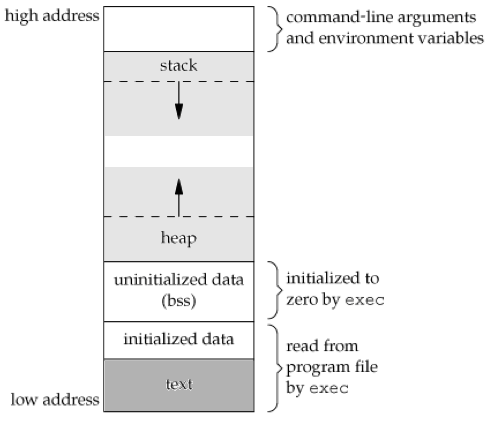
\includegraphics[angle=-90,scale=0.8]{pics/process9.eps}
\end{center}



\subsection{The {\tt main} function}
\vspace{.25in}
\small
\setlength{\unitlength}{1mm}
\begin{center}
	\begin{picture}(150,10)
		\thinlines
		\put(0,0){\framebox(130,10){}}
		\put(10,5){{\tt int main(int {\em argc}, char **{\em argv});}}
	\end{picture}
\end{center}
\Normalsize
\vspace{.25in}
\begin{itemize}
	\item C program started by kernel (by one of the {\tt exec} functions)
	\item special startup routine called by kernel which sets up things for {\tt main} (or whatever entrypoint is defined)
	\item {\tt argc} is a count of the number of command line arguments (including
		the command itself)
	\item {\tt argv} is an array of pointers to the arguments
	\item it is guaranteed by both ANSI C and POSIX.1 that {\tt argv[argc] == NULL}
\end{itemize}

\subsection{Process Creation}
On Linux:
\begin{verbatim}
$ cc -Wall entry.c
$ readelf -h a.out | more
ELF Header:
[...]
  Entry point address:               0x400460
  Start of program headers:          64 (bytes into file)
  Start of section headers:          4432 (bytes into file)
$ objdump -d a.out
[...]
0000000000400460 <_start>:
  400460:       31 ed                   xor    %ebp,%ebp
  400462:       49 89 d1                mov    %rdx,%r9
[...]
$
\end{verbatim}

\subsection{Process Creation}
On Linux:
\begin{verbatim}
$ cc -e foo entry.c
$ ./a.out
Foo for the win!
Memory fault
$ cc -e bar entry.c
$ ./a.out
bar rules!
$ echo $?
1
$ cc entry.c
$ ./a.out
Hooray main!
$ echo $?
13
$
\end{verbatim}

\subsection{Process Termination}
There are 8 ways for a process to terminate.
\\

Normal termination:
\begin{itemize}
	\item return from {\tt main}
	\item calling {\tt exit}
	\item calling {\tt \_exit} (or {\tt\_Exit})
	\item return of last thread from its start routine
	\item calling {\tt pthread\_exit} from last thread
\end{itemize}
\vspace{.25in}
Abnormal termination:
\begin{itemize}
	\item calling {\tt abort}
	\item terminated by a signal
	\item response of the last thread to a cancellation request
\end{itemize}

\subsection{{\tt exit(3)} and {\tt \_exit(2)}}
\small
\setlength{\unitlength}{1mm}
\begin{center}
	\begin{picture}(150,40)
		\thinlines
		\put(0,0){\framebox(130,40){}}
		\put(10,35){{\tt \#include <stdlib.h>}}
		\put(10,29){{\tt void exit(int {\em status});}}
		\put(10,24){{\tt void \_Exit(int {\em status});}}
		\put(10,13){{\tt \#include <unistd.h>}}
		\put(10,8){{\tt void \_exit(int {\em status});}}
	\end{picture}
\end{center}
\Normalsize
\vspace{.5in}
\begin{itemize}
	\item {\tt \_exit} and {\tt \_Exit}
		\begin{itemize}
			\item return to the kernel immediately
			\item {\tt \_exit} required by POSIX.1
			\item {\tt \_Exit} required by ISO C99
			\item synonymous on Unix
		\end{itemize}
	\item {\tt exit} does some cleanup and then returns
	\item both take integer argument, aka {\em exit status}
\end{itemize}

\subsection{{\tt atexit(3)}}
\small
\setlength{\unitlength}{1mm}
\begin{center}
	\begin{picture}(150,20)
		\thinlines
		\put(0,0){\framebox(130,20){}}
		\put(10,13){{\tt \#include <stdlib.h>}}
		\put(10,5){{\tt int atexit(void (*func)({\em void}));}}
	\end{picture}
\end{center}
\Normalsize
\vspace{.5in}
\begin{itemize}
	\item Registers a function with a signature of {\tt void
		funcname(void)} to be called at exit
	\item Functions invoked in reverse order of registration
	\item Same function can be registered more than once
	\item Extremely useful for cleaning up open files,
		freeing certain resources, etc.
\end{itemize}

{\tt exit-handlers.c}

\subsection{Lifetime of a UNIX Process}
\begin{center}
	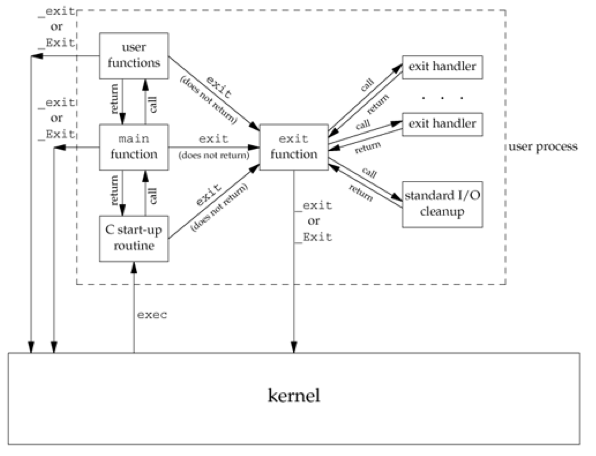
\includegraphics[angle=-90,scale=0.8]{pics/lifetime6.eps}
\end{center}

\subsection{Environment List}
Environment variables are stored in a global array of pointers:
\\

\verb+      extern char **environ;+
\\

The list is {\tt null} terminated.
\\

These can also be accessed by:
\vspace{.25in}
\small
\setlength{\unitlength}{1mm}
\begin{center}
	\begin{picture}(150,35)
		\thinlines
		\put(0,0){\framebox(130,35){}}
		\put(10,30){{\tt \#include <stdlib.h>}}
		\put(10,18){{\tt char *getenv(const char *{\em name});}}
		\put(10,13){{\tt int putenv(const char *{\em string});}}
		\put(10,8){{\tt int setenv(const char *{\em name}, const char *{\em value}, int {\em rewrite});}}
		\put(10,3){{\tt void unsetenv(cont char *{\em name});}}
	\end{picture}
\end{center}
\Normalsize

\subsection{Memory Allocation}
\small
\setlength{\unitlength}{1mm}
\begin{center}
	\begin{picture}(150,40)
		\thinlines
		\put(0,0){\framebox(130,40){}}
		\put(10,35){{\tt \#include <stdlib.h>}}
		\put(10,28){{\tt void *malloc(size\_t {\em size});}}
		\put(10,23){{\tt void *calloc(size\_t {\em nobj}, size\_t {\em size});}}
		\put(10,18){{\tt void *realloc(void *{\em ptr}, size\_t {\em newsize});}}
		\put(10,13){{\tt void *alloca(size\_t {\em size});}}
		\put(10,5){{\tt void free(void *{\em ptr});}}
	\end{picture}
\end{center}
\Normalsize
\begin{itemize}
	\item {\em malloc} -- initial value is indeterminate.
	\item {\em calloc} -- initial value set to all zeros.
	\item {\em realloc} -- changes size of previously allocated area. Initial
		value of any additional space is indeterminate.
	\item {\em alloca} -- allocates memory on stack
\end{itemize}

\subsection{Process limits}
\begin{verbatim}
$ ulimit -a
time(cpu-seconds)    unlimited
file(blocks)         unlimited
coredump(blocks)     unlimited
data(kbytes)         262144
stack(kbytes)        2048
lockedmem(kbytes)    249913
memory(kbytes)       749740
nofiles(descriptors) 128
processes            160
vmemory(kbytes)      unlimited
sbsize(bytes)        unlimited
$
\end{verbatim}

\subsection{{\tt getrlimit(2)} and {\tt setrlimit(2)}}
\small
\setlength{\unitlength}{1mm}
\begin{center}
	\begin{picture}(150,25)
		\thinlines
		\put(0,0){\framebox(130,25){}}
		\put(10,20){{\tt \#include <sys/resource.h>}}
		\put(10,12){{\tt int getrlimit(int {\em resouce}, struct rlimit *{\em rlp});}}
		\put(10,8){{\tt int setrlimit(int {\em resouce}, const struct rlimit *{\em rlp});}}
	\end{picture}
\end{center}
\Normalsize
Changing resource limits follows these rules:
\begin{itemize}
	\item a {\em soft limit} can be changed by any process to a value less
		than or equal to its hard limit
	\item any process can lower its {\em hard limit} greater than or equal to
		its soft limit
	\item only superuser can raise {\em hard limits}
	\item changes are per process only (which is why {\tt ulimit} is a
		shell built-in)
\end{itemize}

\subsection{Process Identifiers}
\small
\setlength{\unitlength}{1mm}
\begin{center}
	\begin{picture}(150,20)
		\thinlines
		\put(0,0){\framebox(130,20){}}
		\put(10,15){{\tt \#include <unistd.h>}}
		\put(10,8){{\tt pid\_t getpid(void);}}
		\put(10,3){{\tt pid\_t getppid(void);}}
	\end{picture}
\end{center}
\Normalsize
\vspace{.25in}
{\em Process ID}'s are guaranteed to be unique and identify a particular executing
process with a non-negative integer.
\vspace{.25in}

Certain processes have fixed, special identifiers. They are:
\begin{itemize}
	\item {\em swapper}, process ID 0 -- responsible for scheduling
    \item {\em init}, process ID 1 -- bootstraps a Unix system, owns orphaned processes
    \item {\em pagedaemon}, process ID 2 -- responsible for the VM system (some Unix systems)
\end{itemize}

\subsection{{\tt fork(2)}}
\small
\setlength{\unitlength}{1mm}
\begin{center}
	\begin{picture}(150,15)
		\thinlines
		\put(0,0){\framebox(130,15){}}
		\put(10,10){{\tt \#include <unistd.h>}}
		\put(10,3){{\tt pid\_t fork(void);}}
	\end{picture}
\end{center}
\Normalsize

{\tt fork(2)} causes creation of a new process.  The new process (child
process) is an exact copy of the calling process (parent process) except for
the following:

\begin{itemize}
	\item The child process has a unique process ID.
	\item The child process has a different parent process ID (i.e., the
		process ID of the parent process).
	\item The child process has its own copy of the parent's descriptors.
	\item The child process' resource utilizations are set to 0.
\end{itemize}

{\bf Note}: no order of execution between child and parent is guaranteed!

\subsection{{\tt fork(2)}}
\begin{center}
	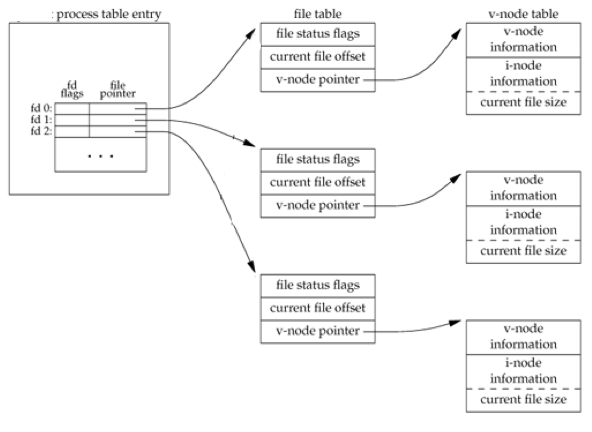
\includegraphics[angle=-90,scale=0.8]{pics/fork1.eps}
\end{center}

\subsection{{\tt fork(2)}}
\begin{center}
	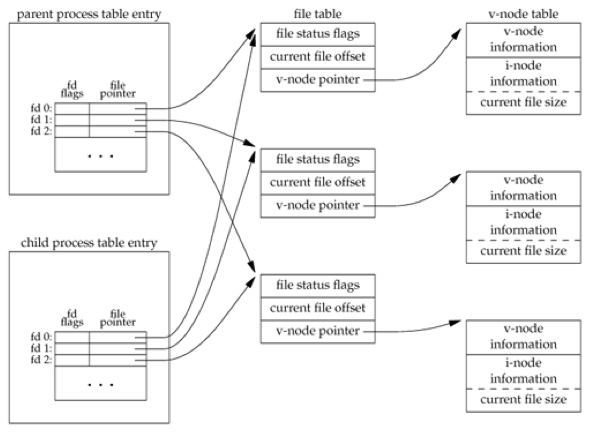
\includegraphics[angle=-90,scale=0.8]{pics/fork2.eps}
\end{center}

\subsection{{\tt fork(2)}}
\begin{verbatim}
$ cc -Wall forkflush.c
$ ./a.out
a write to stdout
before fork
pid = 12149, glob = 7, var = 89
pid = 12148, glob = 6, var = 88
$ ./a.out | cat
a write to stdout
before fork
pid = 12153, glob = 7, var = 89
before fork
pid = 12151, glob = 6, var = 88
$
\end{verbatim}

\subsection{The {\tt exec(3)} functions}
\small
\setlength{\unitlength}{1mm}
\begin{center}
	\begin{picture}(220,50)
		\thinlines
		\put(0,0){\framebox(200,50){}}
		\put(10,45){{\tt \#include <unistd.h>}}
		\put(10,38){{\tt int execl(const char *{\em pathname}, const char *{\em arg0}, ... /* (char *) 0 */);}}
		\put(10,31){{\tt int execv(const char *{\em pathname}, char * const {\em argvp[]});}}
		\put(10,24){{\tt int execle(const char *{\em pathname}, const char *{\em arg0}, ... /* (char *) 0, char
*const {\em envp[]} */ );}}
		\put(10,17){{\tt int execve(const char *{\em pathname}, char * const {\em argvp[]}, char * const {\em envp[]});}}
		\put(10,10){{\tt int execlp(const char *{\em filename}, const char *{\em arg0}, ... /* (char *) 0 */);}}
		\put(10,3){{\tt int execvp(const char *{\em filename}, char *const {\em argv[]});}}
	\end{picture}
\end{center}
\Normalsize

The {\tt exec()} family of functions are used to completely replace a running
process with a a new executable.
\begin{itemize}
	\item if it has a v in its name, argv's are a vector: {\tt const * char argv[]}
	\item if it has an l in its name, argv's are a list: {\tt const char *arg0, ... /* (char *) 0 */}
	\item if it has an e in its name, it takes a {\tt char * const envp[]} array of environment variables
	\item if it has a p in its name, it uses the {\tt PATH} environment variable to search for the file
\end{itemize}

\subsection{{\tt wait(2)} and {\tt waitpid(2)}}
\small
\setlength{\unitlength}{1mm}
\begin{center}
	\begin{picture}(150,40)
		\thinlines
		\put(0,0){\framebox(150,40){}}
		\put(10,35){{\tt \#include <sys/types.h>}}
		\put(10,30){{\tt \#include <sys/wait.h>}}
		\put(10,23){{\tt pid\_t wait(int *{\em status});}}
		\put(10,18){{\tt pid\_t waitpid(pid\_t {\em wpid}, int *{\em status}, int {\em options});}}
		\put(10,13){{\tt pid\_t wait3(int *{\em status}, int {\em options}, struct rusage *{\em rusage});}}
		\put(10,8){{\tt pid\_t wait4(pid\_t {\em wpid}, int *{\em status}, int {\em options}, struct rusage *{\em rusage});}}
	\end{picture}
\end{center}
\Normalsize

A parent that calls {\tt wait(2)} or {\tt waitpid(2)} can:

\begin{itemize}
	\item block (if all of its children are still running)
	\item return immediately with the termination status of a child
	\item return immediately with an error
\end{itemize}

\newpage
\vspace*{\fill}
\begin{center}
  \Hugesize
    Lecture 06
	\hspace*{5mm}\blueline\\ [1em]
	Process Groups, Sessions, Signals
  \Normalsize
\end{center}
\vspace*{\fill}

\subsection{Login Process}
Let's revisit the process relationships for a login:
\vspace*{\fill}
\begin{center}
\begin{tabular}[width=.75\texwidth]{l c l l }
kernel & $\Rightarrow$ & init(8) & \# explicit creation \\
\\
init(8) & $\Rightarrow$ & getty(8) & \# fork(2) \\
\\
getty(8) & $\Rightarrow$ & login(1) & \# exec(3) \\
\\
login(1) & $\Rightarrow$ & \verb+$SHELL+ & \# exec(3) \\
\\
\verb+$SHELL+ & $\Rightarrow$ & ls(1) & \# fork(2) + exec(3) \\
\end{tabular}
\end{center}
\vspace*{\fill}

\subsection{Login Process}
\vspace*{\fill}
\begin{center}
\begin{tabular}[width=.75\texwidth]{l c l}
init(8) & \# PID 1, PPID 0, EUID 0\\
\\
getty(8) & \# PID {\em N}, PPID 1, EUID 0\\
\\
login(1) & \# PID {\em N}, PPID 1, EUID 0\\
\\
\verb+$SHELL+ & \# PID {\em N}, PPID 1, EUID {\em U}\\
\\
ls(1) & \# PID {\em M}, PPID {\em N}, EUID {\em U}\\
\\
\end{tabular}
\vspace*{\fill}
\end{center}
\begin{center}
\verb+pstree -hapun | more+
\end{center}

\subsection{Process Groups}
\small
\setlength{\unitlength}{1mm}
\begin{center}
	\begin{picture}(150,30)
		\thinlines
		\put(0,0){\framebox(130,25){}}
		\put(10,20){{\tt \#include <unistd.h>}}
		\put(10,13){{\tt pid\_t getpgrp(void);}}
		\put(10,8){{\tt pid\_t getpgid(pid\_t {\em pid});}}
		\put(55,3){Returns: process group ID if OK, -1 otherwise}
	\end{picture}
\end{center}
\Normalsize
\begin{itemize}
	\item in addition to having a PID, each process also
		belongs to a process group (collection of processes
		assocaited with the same job / terminal)
	\item each process group has a unique process group ID
	\item process group IDs (like PIDs) are positive integers and can
		be stored in a {\tt pid\_t} data type
	\item each process group can have a process group leader
		\begin{itemize}
			\item leader identified by its process group ID == PID
			\item leader can create a new process group, create processes in the group
		\end{itemize}
	\item a process can set its (or its children's) process group using {\tt setpgid(2)}
\end{itemize}

\subsection{Process Groups}
\begin{center}
	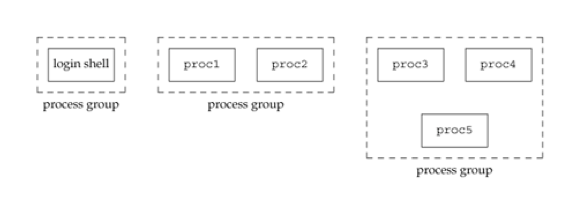
\includegraphics[angle=-90,scale=0.8]{pics/session3.eps}
\end{center}

{\em init} $\Rightarrow$ {\em login shell}
\begin{verbatim}
$ proc1 | proc2 &
[1] 10306
$ proc3 | proc4 | proc5

\end{verbatim}

\subsection{Process Groups and Sessions}
\small
\setlength{\unitlength}{1mm}
\begin{center}
	\begin{picture}(150,30)
		\thinlines
		\put(0,0){\framebox(130,22){}}
		\put(10,18){{\tt \#include <unistd.h>}}
		\put(10,10){{\tt pid\_t setsid(void);}}
		\put(30,5){Returns: process group ID if OK, -1 otherwise}
	\end{picture}
\end{center}
\Normalsize
A session is a collection of one or more process groups. \\

If the calling process is not a process group leader, this
function creates a new session.  Three things happen:
\begin{itemize}
	\item the process becomes the session leader of this new session
	\item the process becomes the process group leader of a new process group
	\item the process has no controlling terminal
\end{itemize}

\subsection{Process Groups}
\begin{center}
	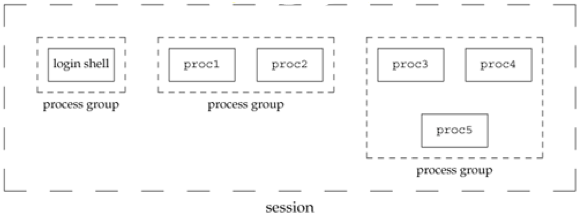
\includegraphics[angle=-90,scale=0.8]{pics/session4.eps}
\end{center}

{\em init} $\Rightarrow$ {\em login shell}
\begin{verbatim}
$ proc1 | proc2 &
[1] 10306
$ proc3 | proc4 | proc5

\end{verbatim}

\subsection{Process Groups and Sessions}
\begin{center}
	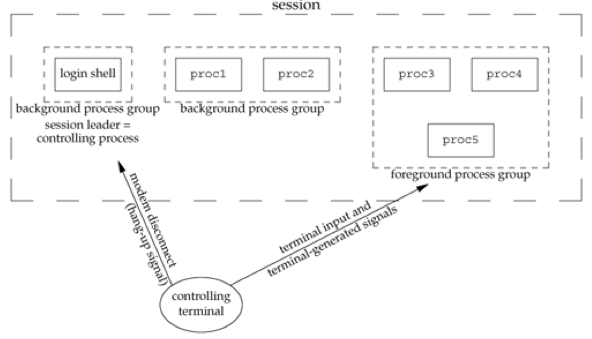
\includegraphics[angle=-90,scale=0.75]{pics/session5.eps}
\end{center}

{\em init} $\Rightarrow$ {\em login shell}
\begin{verbatim}
$ proc1 | proc2 &
[1] 10306
$ proc3 | proc4 | proc5
\end{verbatim}


\subsection{Process Groups and Sessions}
\begin{center}
	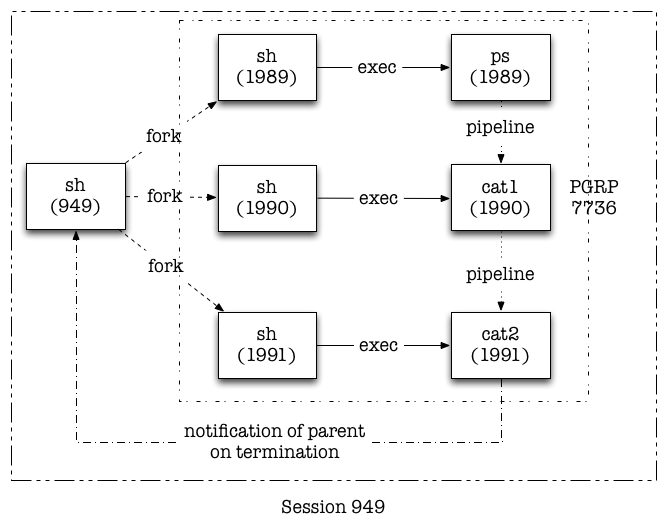
\includegraphics[angle=-90,scale=0.42]{pics/pscat.eps}
\end{center}
\begin{verbatim}
$ ps -o pid,ppid,pgid,sess,comm | ./cat1 | ./cat2
  PID  PPID  PGRP  SESS COMMAND
 1989   949  7736   949 ps
 1990   949  7736   949 cat1
 1988   949  7736   949 cat2
  949 21401   949   949 sh
\end{verbatim}


\subsection{Job Control}
\begin{center}
	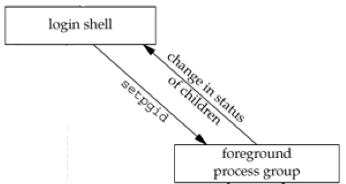
\includegraphics[angle=-90,scale=0.75]{pics/jc4.eps}
\end{center}
\addvspace{.5in}
\begin{verbatim}
$ ps -o pid,ppid,pgid,sess,comm
  PID  PPID  PGRP  SESS COMMAND
24251 24250 24251 24251 ksh
24620 24251 24620 24251 ps
$ echo $?
0
$
\end{verbatim}

\subsection{Job Control}
\begin{center}
	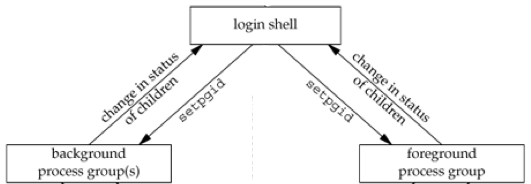
\includegraphics[angle=-90,scale=0.75]{pics/jc2.eps}
\end{center}
\begin{verbatim}
$ dd if=/dev/zero of=/dev/null bs=512 count=2048000 >/dev/null 2>&1 &
[1]	24748
$ ps -o pid,ppid,pgid,sess,comm
  PID  PPID  PGRP  SESS COMMAND
24251 24250 24251 24251 ksh
24748 24251 24748 24251 dd
24750 24251 24750 24251 ps
$
[1] +  Done     dd if=/dev/zero of=/dev/null bs=512 count=2048000 >/dev/null 2>&1 &
$
\end{verbatim}

\subsection{Job Control}
\begin{center}
	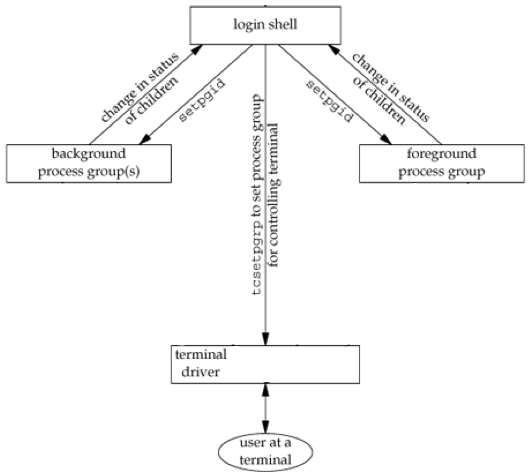
\includegraphics[angle=-90,scale=0.75]{pics/jc6.eps}
\end{center}

\subsection{Job Control}
\begin{center}

\newsavebox\fgio
\begin{lrbox}{\fgio}
	\begin{minipage}[t]{\textwidth}
		\begin{verbatim}
$ cat >file
Input from terminal,
Output to terminal.
^D
$ cat file
Input from terminal,
Output to terminal.
$ cat >/dev/null
Input from terminal,
Output to /dev/null.
Waiting forever...
Or until we send an interrupt signal.
^C
$
\end{verbatim}
	\end{minipage}
\end{lrbox}

\renewcommand{\tabularxcolumn}[1]{>{\arraybackslash}m{#1}}
\begin{tabularx}{\textwidth}{l r }
\begin{minipage}[b]{0.5\textwidth}
\usebox\fgio
\end{minipage} &
		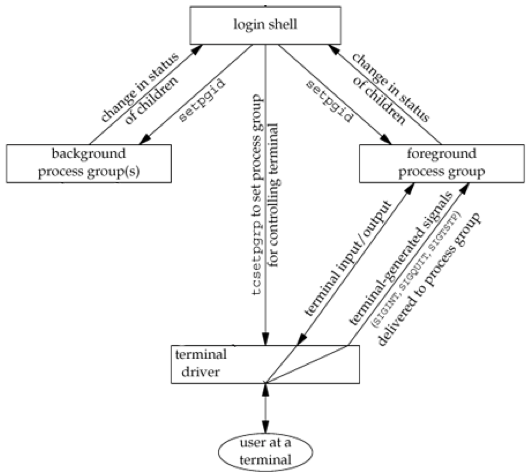
\includegraphics[angle=-90,scale=0.6]{pics/jc5.eps}
	\end{tabularx}
\end{center}

\subsection{Job Control}
\begin{center}

\newsavebox\bgio
\begin{lrbox}{\bgio}
	\begin{minipage}[t]{\textwidth}
		\begin{verbatim}
$ cat file &
[1]	2056
$ Input from terminal,
Output to terminal.

[1] +  Done             cat file &
$ stty tostop
$ cat file &
[1]	4655
$
[1] + Stopped(SIGTTOU)  cat file &
$ fg
cat file
Input from terminal,
Output to terminal.
$
\end{verbatim}
	\end{minipage}
\end{lrbox}

\renewcommand{\tabularxcolumn}[1]{>{\arraybackslash}m{#1}}
\begin{tabularx}{\textwidth}{l r }
\begin{minipage}[b]{0.5\textwidth}
\usebox\bgio
\end{minipage} &
		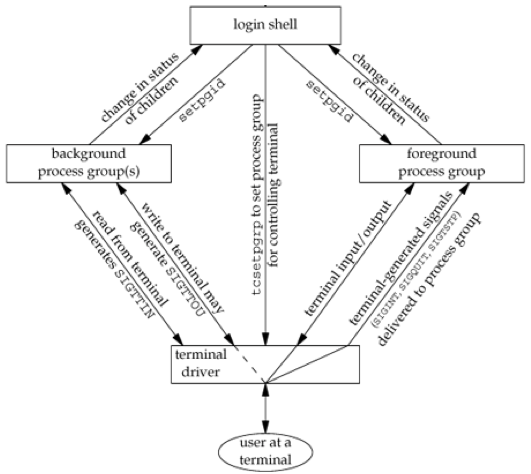
\includegraphics[angle=-90,scale=0.6]{pics/jc1.eps}
	\end{tabularx}
\end{center}

\subsection{Signal Concepts}

Signals are a way for a process to be notified of asynchronous events. Some
examples:

\begin{itemize}
	\item a timer you set has gone off ({\tt SIGALRM})
	\item some I/O you requested has occurred ({\tt SIGIO})
	\item a user resized the terminal "window" ({\tt SIGWINCH})
	\item a user disconnected from the system ({\tt SIGHUP})
	\item ...
\end{itemize}

See also: {\tt signal(2)/signal(3)/signal(7)} (note: these man pages vary
significantly across platforms!)


\subsection{Signal Concepts}
Besides the asynchronous events listed previously, there are many ways to
generate a signal:

\begin{itemize}
	\item terminal generated signals (user presses a key combination which causes
		the terminal driver to generate a signal)
	\item hardware exceptions (divide by 0, invalid memory references, etc)
	\item {\tt kill(1)} allows a user to send any signal to any process (if the
		user is the owner or superuser)
	\item {\tt kill(2)} (a system call, not the unix command) performs the
		same task
	\item software conditions (other side of a pipe no longer exists, urgent data
		has arrived on a network file descriptor, etc.)
\end{itemize}

\subsection{{\tt kill(2)} and {\tt raise(3)}}
\small
\setlength{\unitlength}{1mm}
\begin{center}
	\begin{picture}(150,27)
		\thinlines
		\put(0,0){\framebox(130,27){}}
		\put(10,22){{\tt \#include <sys/types.h>}}
		\put(10,17){{\tt \#include <signal.h>}}
		\put(10,10){{\tt int kill(pid\_t {\em pid}, int {\em signo});}}
		\put(10,5){{\tt int raise(int {\em signo});}}
	\end{picture}
\end{center}
\Normalsize

\begin{itemize}
	\item {\em pid $>$ 0} -- signal is sent to the process whose PID is {\tt pid}
	\item {\em pid == 0} -- signal is sent to all processes whose process
		group ID equals the process group ID of the sender
	\item {\em pid == -1} -- POSIX.1 leaves this undefined, BSD defines it
		(see {\tt kill(2)})
\end{itemize}

\subsection{Signal Concepts}
Once we get a signal, we can do one of several things:

\begin{itemize}
	\item Ignore it. (note: there are some signals which we CANNOT or SHOULD NOT
		ignore)
	\item Catch it. That is, have the kernel call a function which we define
		whenever the signal occurs.
	\item Accept the default. Have the kernel do whatever is defined as the
		default action for this signal
\end{itemize}

\subsection{{\tt signal(3)}}
\small
\setlength{\unitlength}{1mm}
\begin{center}
	\begin{picture}(150,22)
		\thinlines
		\put(0,0){\framebox(130,22){}}
		\put(10,17){{\tt \#include <signal.h>}}
		\put(10,10){{\tt void (*signal(int {\em signo}, void (*func)(int)))(int);}}
		\put(30,3){Returns: previous disposition of signal if OK, {\tt SIG\_ERR} otherwise}
	\end{picture}
\end{center}
\Normalsize
{\em func} can be:
\begin{itemize}
	\item {\tt SIG\_IGN} which requests that we ignore the signal {\tt signo}
	\item {\tt SIG\_DFL} which requests that we accept the default action for signal {\tt signo}
	\item or the address of a function which should catch or handle a signal
\end{itemize}

\subsection{Interrupted System Calls}

Some system calls can block for long periods of time (or forever). These
include things like:

\begin{itemize}
	\item {\tt read(2)}s from files that can block (pipes, networks, terminals)
	\item {\tt write(2)} to the same sort of files
	\item {\tt open(2)} of a device that waits until a condition occurs (for example, a modem)
	\item {\tt pause(3)}, which purposefully puts a process to sleep until a signal occurs
	\item certain {\tt ioctl(3)}s
	\item certain IPC functions
\end{itemize}

Catching a signal during execution of one of these calls traditionally led
to the process being aborted with an errno return of {\tt EINTR}.

\newpage
\vspace*{\fill}
\begin{center}
  \Hugesize
    Lecture 07
	\hspace*{5mm}\blueline\\ [1em]
	Interprocess Communication
  \Normalsize
\end{center}
\vspace*{\fill}

\subsection{Pipes: {\tt pipe(2)}}
\small
\setlength{\unitlength}{1mm}
\begin{center}
	\begin{picture}(150,22)
		\thinlines
		\put(0,0){\framebox(130,22){}}
		\put(10,17){{\tt \#include <unistd.h>}}
		\put(10,10){{\tt int pipe(int {\em filedes[2]});}}
		\put(80,3){Returns: 0 if OK, -1 otherwise}
	\end{picture}
\end{center}
\Normalsize
\begin{itemize}
	\item oldest and most common form of UNIX IPC
	\item half-duplex (on some versions full-duplex)
	\item can only be used between processes that have a common ancestor
	\item can have multiple readers/writers ({\tt PIPE\_BUF} bytes are
		guaranteed to not be interleaved)
\end{itemize}
\vspace{.5in}

Behavior after closing one end:
\begin{itemize}
	\item {\tt read(2)} from a pipe whose write end has been closed returns 0
		after all data has been read
	\item {\tt write(2)} to a pipe whose read end has been closed generates
		{\tt SIGPIPE} signal.  If caught or ignored, {\tt write(2)} returns an
		error and sets {\tt errno} to {\tt EPIPE}.
\end{itemize}

\subsection{Pipes: {\tt popen(3)} and {\tt pclose(3)}}
\small
\setlength{\unitlength}{1mm}
\begin{center}
	\begin{picture}(150,40)
		\thinlines
		\put(0,0){\framebox(130,40){}}
		\put(10,35){{\tt \#include <stdio.h>}}
		\put(10,28){{\tt FILE *popen(const char *{\em cmd}, const char *{\em type});}}
		\put(62,21){Returns: file pointer if OK, {\tt NULL} otherwise}
		\put(10,10){{\tt int pclose(FILE *{\em fp});}}
		\put(55,3){Returns: termination status {\em cmd} or -1 on error}
	\end{picture}
\end{center}
\Normalsize
\vspace{.5in}
\begin{itemize}
	\item historically implemented using unidirectional pipe (nowadays
		frequently implemented using sockets or full-duplex pipes)
	\item {\em type} one of ``r'' or ``w'' (or ``r+'' for
		bi-directional communication, if available)
	\item {\em cmd} passed to {\tt /bin/sh -c}
\end{itemize}

\subsection{FIFOs: {\tt mkfifo(2)}}
\small
\setlength{\unitlength}{1mm}
\begin{center}
	\begin{picture}(150,22)
		\thinlines
		\put(0,0){\framebox(130,22){}}
		\put(10,17){{\tt \#include <sys/stat.h>}}
		\put(10,10){{\tt int mkfifo(const char *{\em path}, mode\_t {\em mode});}}
		\put(80,3){Returns: 0 if OK, -1 otherwise}
	\end{picture}
\end{center}
\Normalsize

\begin{itemize}
	\item aka ``named pipes''
	\item allows unrelated processes to communicate
	\item just a type of file -- test for using {\tt S\_ISFIFO(st\_mode)}
	\item {\em mode} same as for {\tt open(2)}
	\item use regular I/O operations (ie {\tt open(2)}, {\tt read(2)}, {\tt
		write(2)}, {\tt unlink(2)} etc.)
	\item used by shell commands to pass data from one shell
			pipeline to another without creating intermediate
			temporary files
\end{itemize}

\subsection{System V IPC}
Three types of IPC originating from System V:
\begin{itemize}
	\item Semaphores
	\item Shared Memory
	\item Message Queues
\end{itemize}
\vspace{.5in}

All three use {\em IPC structures}, referred to by an {\em identifier} and a
{\em key}; all three are (necessarily) limited to communication between
processes on one and the same host.
\\

Since these structures are not known by name, special system calls ({\tt
msgget(2)}, {\tt semop(2)}, {\tt shmat(2)}, etc.) and special userland
commands ({\tt ipcrm(1)}, {\tt ipcs(1)}, etc.) are necessary.

\subsection{Sockets: {\tt socketpair(2)}}
\small
\setlength{\unitlength}{1mm}
\begin{center}
	\begin{picture}(150,22)
		\thinlines
		\put(0,0){\framebox(130,22){}}
		\put(10,17){{\tt \#include <sys/socket.h>}}
		\put(10,10){{\tt int socketpair(int {\em d}, int {\em type}, int {\em protocol}, int *{\em sv});}}
	\end{picture}
\end{center}
\Normalsize

The {\tt socketpair(2)} call creates an unnamed pair of connected sockets in
the specified domain {\tt d}, of the specified {\em type}, and using the
optionally specified {\em protocol}.
\\

The descriptors used in referencing the new sockets are returned in {\em
sv[0]} and {\em sv[1]}.  The two sockets are indistinguishable.
\\

{\tt This call is currently implemented only for the UNIX domain.}

\subsection{Sockets: {\tt socket(2)}}
\small
\setlength{\unitlength}{1mm}
\begin{center}
	\begin{picture}(150,22)
		\thinlines
		\put(0,0){\framebox(130,22){}}
		\put(10,17){{\tt \#include <sys/socket.h>}}
		\put(10,10){{\tt int socket(int {\em domain}, int {\em type}, int {\em protocol});}}
	\end{picture}
\end{center}
\Normalsize
Some of the currently supported domains are:
\\

\small
\begin{tabular}{| l | l |}
	\hline
	{\bf Domain} & {\bf Description} \\
	\hline
	{\tt PF\_LOCAL} 	& 	local (previously UNIX) domain protocols \\
	{\tt PF\_INET}		&	ARPA Internet protocols \\
	{\tt PF\_INET6}		&	ARPA IPv6 (Internet Protocol version 6) protocols \\
	{\tt PF\_ARP}		&	RFC 826 Ethernet Address Resolution Protocol\\
	{\tt ...}		&	...\\
	\hline
\end{tabular}
\Normalsize
\vspace{.5in}

Some of the currently defined types are:
\\

\small
\begin{tabular}{| l | l |}
	\hline
	{\bf Type}		&	{\bf Description} \\
	\hline
	{\tt SOCK\_STREAM}	&	sequenced, reliable, two-way connection based byte streams \\
	{\tt SOCK\_DGRAM}	&	connectionless, unreliable messages of a fixed (typically small)
							maximum length \\
	{\tt SOCK\_RAW}		&	access to internal network protocols and interfaces \\
	{\tt ...}		&	... \\
	\hline
\end{tabular}
\Normalsize

\subsection{Sockets: Datagrams in the UNIX/LOCAL domain}
\begin{itemize}
	\item create socket using {\tt socket(2)}
	\item attach to a socket using {\tt bind(2)}
	\item binding a name in the UNIX domain creates a socket in the file system
	\item both processes need to agree on the name to use
	\item these files are only used for rendezvous, not for message delivery
		once a connection has been established
	\item sockets must be removed using {\tt unlink(2)}
\end{itemize}

\subsection{Sockets: Datagrams in the Internet Domain}
\begin{itemize}
	\item Unlike UNIX domain names, Internet socket names are not entered into
		the file system and, therefore, they do not have to be unlinked after the
		socket has been closed.
	\item The local machine address for a socket can be any valid network address
		of the machine, if it has more than one, or it can be the wildcard value
		{\tt INADDR\_ANY}.
	\item ``well-known'' ports (range 1 - 1023) only available to super-user
	\item request any port by calling {\tt bind(2)} with a port number of 0
	\item determine used port number (or other information) using {\tt
		getsockname(2)}
	\item convert between network byteorder and host byteorder using {\tt
		htons(3)} and {\tt ntohs(3)} (which may be noops)
\end{itemize}

\subsection{Sockets: Connections using stream sockets}
\begin{itemize}
	\item connections are asymmetrical:  one process requests a connection,
		the other process accepts the request
	\item one socket is created for each accepted request
	\item mark socket as willing to accept connections using {\tt listen(2)}
	\item pending connections are then {\tt accept(2)}ed
	\item {\tt accept(2)} will block if no connections are available
	\item {\tt select(2)} to check if connection requests are pending
\end{itemize}

\newpage
\vspace*{\fill}
\begin{center}
  \Hugesize
	Lecture 08
	\hspace*{5mm}\blueline\\ [1em]
	UNIX Tools
  \Normalsize
\end{center}
\vspace*{\fill}

\subsection{Software Development Tools}
UNIX Userland is an IDE -- essential tools that follow the paradigm of ``Do
one thing, and do it right'' can be combined. \\

The most important tools are:
\begin{itemize}
	\item \verb+$EDITOR+
	\item the compiler toolchain
	\item {\tt gdb(1)} -- debugging your code
	\item {\tt make(1)} -- project build management, maintain program
		dependencies
	\item {\tt diff(1)} and {\tt patch(1)} -- report and apply differences
		between files
	\item {\tt cvs(1)}, {\tt svn(1)}, {\tt git(1)} etc. -- distributed project management,
		 version control
\end{itemize}

\subsection{Preprocessing}

The compiler usually performs preprocessing (via {\tt cpp(1)}), compilation
({\tt cc(1)}), assembly ({\tt as(1)}) and linking ({\tt ld(1)}).

\begin{verbatim}
$ cd compilechain
$ cat hello.c
$ man cpp
$ cpp hello.c hello.i
$ file hello.i
$ man cc
$ cc -v -E hello.c > hello.i
$ more hello.i
$ cc -v -DFOOD=\"Avocado\" -E hello.c > hello.i.2
$ diff -bu hello.i hello.i.2
\end{verbatim}

\subsection{Compilation}

The compiler usually performs preprocessing (via {\tt cpp(1)}), compilation
({\tt cc(1)}), assembly ({\tt as(1)}) and linking ({\tt ld(1)}).

\begin{verbatim}
$ more hello.i
$ cc -v -S hello.i > hello.s
$ file hello.s
$ more hello.s
\end{verbatim}

\subsection{Assembly}

The compiler usually performs preprocessing (via {\tt cpp(1)}), compilation
({\tt cc(1)}), assembly ({\tt as(1)}) and linking ({\tt ld(1)}).

\begin{verbatim}
$ as -o hello.o hello.s
$ file hello.o
$ cc -v -c hello.s
$ objdump -d hello.o
[...]
\end{verbatim}

\subsection{Linking}

The compiler usually performs preprocessing (via {\tt cpp(1)}), compilation
({\tt cc(1)}), assembly ({\tt as(1)}) and linking ({\tt ld(1)}).

\begin{verbatim}
$ ld hello.o
[...]
$ ld hello.o -lc
[...]
$ cc -v hello.o
[...]
$ ld -dynamic-linker /lib64/ld-linux-x86-64.so.2 \
        /usr/lib/x86_64-linux-gnu/crt1.o         \
        /usr/lib/x86_64-linux-gnu/crti.o hello.o \
        -lc /usr/lib/x86_64-linux-gnu/crtn.o
$ file a.out
$ ./a.out
\end{verbatim}

\subsection{{\tt gdb(1)}}

The purpose of a debugger such as {\tt gdb(1)} is to allow you to see what is
going on ``inside'' another program while it executes -- or what another
program was doing at the moment it crashed. {\tt gdb} allows you to

\begin{itemize}
	\item make your program stop on specified conditions (for example by
		setting {\em breakpoints})
	\item examine what has happened, when your program has stopped (by looking
		at the {\em backtrace}, inspecting the value of certain variables)
	\item inspect control flow (for example by {\em stepping} through the
		program)
\end{itemize}
\vspace{.25in}
Other interesting things you can do:

\begin{itemize}
	\item examine stack frames: {\em info frame}, {\em info locals}, {\em info
		args}
	\item examine memory: {\em x}
	\item examine assembly: {\em disassemble func}
\end{itemize}

\subsection{{\tt make(1)}}
{\tt make(1)} is a command generator and build utility. Using a
description file (usually {\em Makefile}) it creates a sequence of
commands for execution by the shell.

\begin{itemize}
	\item used to sort out dependency relations among files
	\item avoids having to rebuild the entire project after modification of a
		single source file
	\item performs {\em selective} rebuilds following a {\em dependency graph}
	\item allows simplification of rules through use of {\em macros} and {\em
		suffixes}, some of which are internally defined
	\item different versions of {\tt make(1)} (BSD make, GNU make, Sys V make,
		...) may differ (among other things) in
		\begin{itemize}
			\item variable assignment and expansion/substitution
			\item including other files
			\item flow control (for-loops, conditionals etc.)
		\end{itemize}
\end{itemize}

\subsection{{\tt diff(1)} and {\tt patch(1)}}
{\tt diff(1)}:
\begin{itemize}
	\item compares files line by line
	\item output may be used to automatically edit a file
	\item can produce human ``readable'' output as well as diff entire
		directory structures
	\item output called a {\em patch}
\end{itemize}

{\tt patch(1)}:
\begin{itemize}
	\item applies a {\tt diff(1)} file (aka {\em patch}) to an original
	\item may back up original file
	\item may guess correct format
	\item ignores leading or trailing ``garbage''
	\item allows for reversing the patch
	\item may even correct context line numbers
\end{itemize}

\subsection{Revision Control}
Version control systems allow you to

\begin{itemize}
	\item collaborate with others
	\item simultaneously work on a code base
	\item keep old versions of files
	\item keep a log of the who, when, what, and why of any changes
	\item perform release engineering by creating {\em branches}
\end{itemize}

\newpage
\vspace*{\fill}
\begin{center}
  \Hugesize
	Lecture 09
	\hspace*{5mm}\blueline\\ [1em]
	Shared Libraries
  \Normalsize
\end{center}
\vspace*{\fill}

\subsection{Shared Libraries}
What is a shared library, anyway?
\begin{itemize}
	\item contains a set of callable C functions (ie, implementation
		of function prototypes defined in {\tt .h} header files)
	\item code is position-independent (ie, code can be executed anywhere
		in memory)
	\item shared libraries can be loaded/unloaded at execution time or at will
	\item libraries may be {\em static} or {\em dynamic}
\end{itemize}
\begin{verbatim}
$ man 3 fprintf
$ grep " fprintf" /usr/include/stdio.h
\end{verbatim}


\subsection{Shared Libraries}
How do shared libraries work?
\begin{itemize}
	\item contents of {\em static} libraries are pulled into the
		executable at link time
	\item contents of {\em dynamic} libraries are used to resolve
		symbols at {\bf link time}, but loaded at {\bf execution time} by the
		{\em dynamic linker}
	\item contents of {\em dynamic} libraries may be loaded at {\bf any
		time} via explicit calls to the dynamic linking loader interface
		functions
\end{itemize}

\subsection{Shared Libraries}
Static libraries:
\begin{itemize}
	\item created by {\tt ar(1)}
	\item usually end in {\tt .a}
	\item contain a symbol table within the archive (see {\tt
		ranlib(1)})
\end{itemize}

Dynamic libraries:
\begin{itemize}
	\item created by the compiler/linker (ie multiple steps)
	\item usually end in {\tt .so}
	\item frequently have multiple levels of symlinks providing
		backwards compatibility / ABI definitions
\end{itemize}

\subsection{Dynamically Linked Shared Libraries}
The link loader needs to know where to find all required shared libraries.
\begin{verbatim}
$ export LD_LIBRARY_PATH=${LD_LIBRARY_PATH}:./lib
$ ldd a.out
[...]
$ ./a.out
[...]
$ mkdir lib2
$ cc -Wall -c -fPIC ldtest1.2.c
$ cc -shared -Wl,-soname,libldtest.so.1 -o lib2/libldtest.so.1.0 ldtest1.2.o ldtest2.o
$ ln -s libldtest.so.1.0 lib2/libldtest.so.1
$ ln -s libldtest.so.1.0 lib2/libldtest.so
$ export LD_LIBRARY_PATH=./lib2:$LD_LIBRARY_PATH
$ ldd a.out  # note: no recompiling!
[...]
$ ./a.out
[...]
\end{verbatim}

\subsection{Dynamically Linked Shared Libraries}
Avoiding {\tt LD\_LIBRARY\_PATH}:
\begin{verbatim}
$ cc -Wall main.o -L./lib -lldtest -Wl,-rpath,./lib
$ echo $LD_LIBRARY_PATH
[...]
$ ldd a.out
[...]
$ ./a.out
[...]
$ unset LD_LIBRARY_PATH
$ ldd a.out
[...]
$ ./a.out
[...]
$
\end{verbatim}

\newpage
\vspace*{\fill}
\begin{center}
  \Hugesize
	Lecture 10
	\hspace*{5mm}\blueline\\ [1em]
	Advanced IO / Encryption in a Nutshell
  \Normalsize
\end{center}
\vspace*{\fill}

\subsection{Nonblocking I/O}
Recall from our lecture on signals that certain system calls can block forever:
\begin{itemize}
	\item {\tt read(2)} from a particular file, if data isn't present (pipes,
		terminals, network devices)
	\item {\tt write(2)} to the same kind of file
	\item {\tt open(2)} of a particular file until a specific condition occurs
	\item {\tt read(2)} and {\tt write(2)} of files that have mandatory
		locking enabled
	\item certain {\tt ioctls(2)}
	\item some IPC functions (such as {\tt sendto(2)} or {\tt recv(2)})
\end{itemize}
\vspace{.25in}
Nonblocking I/O lets us issue an I/O operation and not have it block forever.
If the operation cannot be completed, return is made immediately with an error
noting that the operating would have blocked ({\tt EWOULDBLOCK} or {\tt EAGAIN}).

\subsection{Advisory Locking}
\small
\setlength{\unitlength}{1mm}
\begin{center}
	\begin{picture}(150,22)
		\thinlines
		\put(0,0){\framebox(130,22){}}
		\put(10,17){{\tt \#include <fcntl.h>}}
		\put(10,10){{\tt int flock(int {\em fd},int {\em operation});}}
		\put(80,3){Returns: 0 if OK, -1 otherwise}
	\end{picture}
\end{center}
\Normalsize
\begin{itemize}
	\item applies or removes an advisory lock on the file associated with
		the file descriptor fd
	\item {\em operation} can be {\tt LOCK\_NB} and any one of:
		\begin{itemize}
			\item {\tt LOCK\_SH}
			\item {\tt LOCK\_EX}
			\item {\tt LOCK\_UN}
		\end{itemize}
	\item locks entire file
\end{itemize}

\subsection{Advisory ``Record'' locking}
\small
\setlength{\unitlength}{1mm}
\begin{center}
	\begin{picture}(180,20)
		\thinlines
		\put(0,0){\framebox(160,20){}}
		\put(10,15){{\tt \#include <unistd.h>}}
		\put(10,7){{\tt int lockf(int {\em fd}, int {\em value}, off\_t {\em size});}}
		\put(100,3){Returns: 0 on success, -1 on error}
	\end{picture}
\end{center}
\Normalsize

{\em value} can be:
\begin{itemize}
	\item {\tt F\_ULOCK} -- unlock locked sections
	\item {\tt F\_LOCK} -- lock a section for exclusive use
	\item {\tt F\_TLOCK} -- test and lock a section for exclusive use
	\item {\tt F\_TEST} -- test a section for locks by other processes
\end{itemize}
\begin{center}
	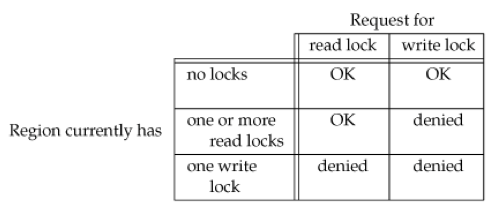
\includegraphics[angle=-90,scale=0.7]{pics/locking.eps}
\end{center}

\subsection{Advisory ``Record'' locking}
Locks are:
\begin{itemize}
	\item released if a process terminates
	\item released if a filedescriptor is closed (!)
	\item not inherited across {\tt fork(2)}
	\item inherited across {\tt exec(2)}
	\item released upon {\tt exec(2)} if close-on-exec is set
\end{itemize}

\subsection{Memory Mapped I/O}
\small
\setlength{\unitlength}{1mm}
\begin{center}
	\begin{picture}(180,30)
		\thinlines
		\put(0,0){\framebox(160,30){}}
		\put(10,25){{\tt \#include <sys/types.h>}}
		\put(10,20){{\tt \#include <sys/mman.h>}}
		\put(10,12){{\tt void *mmap(void *{\em addr}, size\_t {\em len}, int {\em prot}, int {\em flags}, int {\em fd}, off\_t {\em offset});}}
		\put(95,3){Returns: pointer to mapped region if OK}
	\end{picture}
\end{center}
\Normalsize
Protection specified for a region:
\begin{itemize}
	\item {\tt PROT\_READ} -- region can be read
	\item {\tt PROT\_WRITE} -- region can be written
	\item {\tt PROT\_EXEC} -- region can be executed
	\item {\tt PROT\_NONE} -- region can not be accessed
\end{itemize}
\vspace{.25in}
{\em flag} needs to be one of
\begin{itemize}
	\item {\tt MAP\_SHARED}
	\item {\tt MAP\_PRIVATE}
	\item {\tt MAP\_COPY}
\end{itemize}
which may be OR'd with other flags (see {\tt mmap(2)} for details).

\subsection{Cryptography}
Cryptography can provide ``security'' in the areas of:
\begin{itemize}
	\item Authenticity
		\begin{itemize}
			\item {\em Is the party I'm talking to actually who I {\em think} it is?}
		\end{itemize}
	\item Accuracy or Integrity
		\begin{itemize}
			\item {\em Is the message I received in fact what was sent?}
		\end{itemize}
	\item Secrecy or Confidentiality
		\begin{itemize}
			\item {\em Did/could anybody else see (parts of) the message?}
		\end{itemize}
\end{itemize}

\subsection{How does encryption work?}
{\em Secrecy}:  Make sure that the data can only be read by those intended.
\begin{itemize}
	\item Alice and Bob agree on a way to transform data
	\item transformed data is sent over insecure channel
	\item Alice and Bob are able to get data out of the transformation
\end{itemize}
\addvspace{.5in}
\begin{center}
	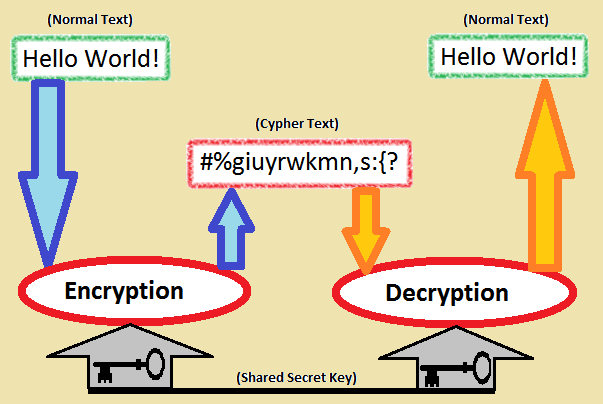
\includegraphics[angle=-90,scale=0.5]{pics/symmetric-key-crypto.eps}
\end{center}

\subsection{Cipher Modes}
Encryption entails transformation of input data (``plain''
or ``clear'' text) into encrypted output data
(``ciphertext'').  Input data is generally transformed
in one of two ways:
\\

{\em Stream Cipher}: each bit on plaintext is combined
with a pseudo-random cipher digit stream (or {\em keystream})
\\

{\em Block Cipher}: fixed-length blocks of plaintext
are transformed into same-sized blocks of ciphertext;
may require padding

\subsection{HW\#4}
\begin{verbatim}
https://www.cs.stevens.edu/~jschauma/631/f16-hw4.html
\end{verbatim}
\begin{verbatim}

To encrypt the contents of the file ’file’ and storing the encrypted out-
put in ’file.enc’:

        aed -e <file >file.enc

To decrypt the contents of that file again:

        aed -d <file.enc

Since aed operates on stdin and stdout, the above two commands could also
be chained:

        cat file | aed -e | aed -d
\end{verbatim}
\Normalsize

\subsection{That's all, folks!}

\begin{center}
	
\includegraphics[angle=-90,scale=0.9]{pics/thats-all-folks.eps}
\end{center}

\end{document}
